\documentclass[fleqn]{NotesClass}

%% Packages
\usepackage[version=4]{mhchem}
\usepackage{csquotes}

% Tikz stuff
\usepackage{tikz}
\tikzset{>=latex}
% External
\usetikzlibrary{external}
\tikzexternalize[prefix=tikz-external/]
%\tikzexternaldisable
% Tikz Feynman
\usepackage[compat=1.1.0]{tikz-feynman}
\tikzfeynmanset{warn luatex=false}
\usepackage{pgfplots}
\usepackage{pgfplotstable}


% Siunitx
\usepackage{siunitx}
\DeclareSIUnit{\fermi}{\femto\meter}
\DeclareSIUnit{\MeV}{\mega\electronvolt}
\DeclareSIUnit{\clight}{\text{\ensuremath{c}}}
\DeclareSIUnit[per-mode=symbol]{\MeVpercsquared}{\MeV\per\clight\squared}
\DeclareSIUnit[per-mode=symbol]{\MeVperc}{\MeV\per\clight}
\DeclareSIUnit{\bohrmagneton}{\ensuremath{\upmu_{\mathrm{B}}}}
\DeclareSIUnit{\nuclearmagneton}{\ensuremath{\upmu_{\mathrm{N}}}}
\DeclareSIUnit{\amu}{u}

% References, should be last things loaded
\usepackage{hyperref}  % Should be loaded second last (cleveref last)
\colorlet{hyperrefcolor}{blue!60!black}
\hypersetup{colorlinks=true, linkcolor=hyperrefcolor, urlcolor=hyperrefcolor}
\usepackage[
capitalize,
nameinlink,
noabbrev
]{cleveref} % Should be loaded last

% My packages
\usepackage{NotesBoxes}
\usepackage{NotesMaths}

\usepackage{ParticlesPackage}
\makeatletter
\newcommand*{\PW}{\ensuremath{\PBASE@wboson}}
\newcommand*{\Peneutral}{\ensuremath{\PBASE@electron}}
\newcommand*{\Palpha}{\ensuremath{\upalpha}}
\makeatother


% Title page info
\title{Relativity, Nuclear, and Particle Physics\\{\Huge---Nuclear Physics}}
\author{Willoughby Seago}
\date{September 20, 2021}
% \subtitle{}
% \subsubtitle{}

% Highlight colour
%\definecolor{highlight}{HTML}{F36619}
\definecolor{darker}{HTML}{933808}
\definecolor{colder}{HTML}{863F86}
\definecolor{tetrad green}{HTML}{A8F31B}
\definecolor{tetrad blue}{HTML}{1BA8F3}
\definecolor{tetrad purple}{HTML}{671BF3}

% Commands
% Particles
\makeatletter
\newcommand{\Pdeuteron}{\ensuremath{\particletypeface{D}}}
\newcommand{\PBASE@pion}{\uppi}
\newcommand{\Ppion}{\ensuremath{\PBASE@pion}}
\newcommand{\Ppionp}{\ensuremath{\Ppion^+}}
\newcommand{\Ppionm}{\ensuremath{\Ppion^-}}
\newcommand{\Ppionzero}{\ensuremath{\Ppion^0}}
\newcommand{\Ppip}{\Ppionp}
\newcommand{\Ppim}{\Ppionm}
\newcommand{\Ppizero}{\Ppionzero}
\newcommand{\PBASE@Delta}{\Updelta}
\newcommand{\PDeltap}{\ensuremath{\PBASE@Delta^+}}
\newcommand{\PDeltazero}{\ensuremath{\PBASE@Delta^0}}
\newcommand{\Pee}{\PBASE@electron}
\makeatother

% Text

% Maths
\newcommand{\e}{\mathrm{e}}
\newcommand{\fermiEnergy}{E_{\mathrm{F}}}

% Include
\includeonly{}

\begin{document}
    \frontmatter
    \titlepage
    \title{Relativity, Nuclear and Particle Physics (Nuclear Physics)}
    \innertitlepage{tikz-external/nucleon-nucleon-interaction.pdf}
    \tableofcontents
    \mainmatter
    
    \chapter{The Big Bang and Virtual Particles}
    \section{The Big Bang}
    13.7 billion years ago the Big Bang occurred.
    About \qty{e-3}{\second} after this the temperature of the universe was \(T \sim \qty{e12}{\kelvin}\).
    At this point the universe was cool enough that protons, \Pp, and neutrons, \Pn, could bind together to form the first nuclei, specifically they formed deuterons, \Pdeuteron, that is proton-neutron pairs which form the nucleus of the deuterium atom, \ce{^2H}.
    This happens in the reaction
    \begin{equation}
        \Pproton + \Pneutron \leftrightharpoons \Pdeuteron + \Pphoton.
    \end{equation}

    There are two things to notice about this.
    First, the photon is needed since the mass of the deuteron is less than the combined mass of the proton and neutron, and this excess energy has to go somewhere.
    Note that it can't go to the kinetic energy of the deuteron since we can always transform to the frame of the deuteron where it has no kinetic energy.
    This reaction is, at this point in time, reversible since there are so many high energy photons flying around that can collide with deuterons and cause them to photodisintegrate into protons and neutrons.
    
    A few seconds after the Big Bang the universe had cooled to \(T \sim \qty{e9}{\kelvin}\).
    At this point there weren't enough high energy photons present to cause the photodisintegration of deuterons and so the reaction is essentially one way:
    \begin{equation}
        \Pproton + \Pneutron \rightarrow \Pdeuteron + \Pphoton.
    \end{equation}
    The energy of most photons at this point is below the \qty{2.22}{\mega\electronvolt} deuteron binding energy.
    
    After deuteron's were produced they underwent further reactions to create the other light nuclei \ce{^3He}, \ce{^4He}, \ce{^6Li}, and \ce{^7Li}.
    These were the only nuclei produced in the Big Bang.
    Originally many scientists thought that all elements were created in the Big Bang.
    Most notably a Russian physicist George Gamow\footnote{Russian, so w is pronounced like v, \textit{gam-ov}}.
    He wrote a paper expressing these ideas with his PhD student Ralph Alpher.
    They decided to also add the name of Gamow's friend, the physicist Hans Bethe\footnote{pronounced \textit{beta}}, simply for the comedic effect of being able to write a paper by Alpher, Bethe and Gamow\footnote{pronounced \textit{alpha}, \textit{beta}, and \textit{gam-ov}}.
    Unfortunately they turned out to be wrong, heavier elements were formed after the big bang in stars and super novae.
    
    The abundance of these lighter elements is some of the earliest evidence that we have for the Big Bang.
    In total Big Bang nucleosynthesis lasted only about 3 minutes.
    It wasn't until approximately 300,000 years after the Big Bang that the universe had cooled enough that electrons could bind to nuclei to form neutral atoms (recall that the binding energy of an electron to a proton, i.e. \ce{^1H}, is only \qty{13.6}{\electronvolt}, much less than the \qty{2.22}{\mega\electronvolt} binding energy of the deuteron).
    At this point the neutral particles in the universe become pretty much transparent to electromagnetic waves and we get the cosmic microwave background radiation.
    
    At this point we ask a question that will motivate much of the following work:
    \begin{important}
        What force binds nuclei together?
    \end{important}
    It can't be the electromagnetic force, protons are positive and neutrons are negative, so at best there is no electromagnetic interaction and at worst they actively repel each other.
    It also can't be gravity, it simply isn't strong enough.
    Both gravity (at least, Newtonian gravity) and the electrostatic force follow inverse square laws, therefore at a given distance the force due to gravity between two nucleons satisfies
    \begin{equation}
        F_Gr^2 = GMm = - (\qty{6.67e-11}{\newton\meter\squared\per\kilogram\squared})(\qty{1.67e-27}{\kilogram})^2 = \qty{1.86e-64}{\newton\meter\squared}
    \end{equation}
    whereas the electrostatic force between two protons satisfies
    \begin{equation}
        F_Er^2 = \frac{e^2}{4\pi\varepsilon_0} = \frac{(\qty{1.6e-19}{\coulomb})^2}{4\pi (\qty{8.85e-12}{\farad\per\meter})} = \qty{2.30e-28}{\newton\meter\squared}.
    \end{equation}
    We can see from this that gravity is a factor of \num{e36} times weaker than the electrostatic force.
    So gravity alone can't be holding together a nucleus of more than one proton.
    
    The answer is that we need a new force, called the \defineindex{strong force} which is strong enough to hold together the nucleus, but doesn't have a noticeable effect on macroscopic scales.
    To understand this force we will need to learn the basic principles of how microscopic particles interact according to quantum mechanics and quantum field theory (QFT)\glossary[acronym]{QFT}{quantum field theory}.
    
    \section{Energy-Time Uncertainty Relation}
    A familiar result from quantum mechanics is that the uncertainty in the energy, \(\Delta E\), of a quantum system is related to the time interval, \(\Delta t\), over which the system changes appreciably:
    \begin{equation}
        \Delta E \Delta t \sim \hbar
    \end{equation}
    Where we use \(\sim\) informally to mean \enquote{is about the same size as}.
    
    A consequence of this is that all unstable states, that is states with a finite lifetime (since decay is certainly an appreciable change) have finite (here meaning nonzero) energy uncertainty.
    We can define the \defineindex{energy width}, \(\Gamma\), which relates this uncertainty to the lifetime, \(\tau\), of the quantum system, by
    \begin{equation}
        \Gamma\tau = \hbar.
    \end{equation}
    When we say \enquote{energy width} what we mean is a measure of the width of the distribution of energy values.
    Since this is usually a Lorentzian distribution by width we mostly mean the full width at half maximum.
    
    A result of this is that only completely stable systems, where \(\tau = \infty\), can have \(\Gamma = \Delta E = 0\).
    
    Another feature of the uncertainty relation is it allows for temporary violation of the conservation of energy over short time periods, \(\Delta t\), energy conservation can be violated by up to \(\Delta E\).
    This allows for effects that would otherwise be impossible.
    
    For example, a laser involves lots of atoms emitting and absorbing photons of the same frequency.
    Since these atoms aren't perfectly still every photon will have some Doppler shift associated with its frequency.
    If atoms could only absorb photons with exactly the same energy that they emit then they would never be able to absorb, instead they can actually absorb within \(\Gamma/2\) of this value, and so can absorb photons from other atoms.
    Since lasers clearly work this is evidence for the uncertainty principle.
    
    Critically while instantaneous energy conservation no longer applies over a sufficiently long period of time energy must still be conserved.
    We can thing of this as \enquote{borrowing} energy from the uncertainty principle and having to pay it back.
    
    \section{Yukawa Exchange Model of Nucleon-Nucleon Interactions}
    In this section we consider nucleon-nucleon interactions.
    Nucleon simply means proton or neutron.
    For simplicity we will focus on \Pn-\Pn{} interactions as this allows us to ignore electromagnetic effects but the same analysis applies to \Pp-\Pn{} and \Pp-\Pp{} interactions.
    
    This model of interaction was developed by Japanese physicist Hideki Yukawa in 1935.
    It posits an \defineindex{exchange particle}, also known as a \define{virtual particle}\index{virtual particle|see{exchange particle}} or \define{field quantum}\index{field quantum|see{exchange particle}}.
    The simplest way to view the interaction is with a Feynman diagram, showing the world lines of the particles involved.
    This is shown for \Pn-\Pn{} in \cref{fig:n-n feynman diagram}.
    
    \begin{figure}
        \tikzsetnextfilename{n-n-interaction}
        \begin{tikzpicture}
            \begin{feynman}
                \vertex (a);
                \vertex[below=of a] (b);
                \vertex (n in 1) at ($(a) + (-2, 0.5)$) {\Pn};
                \vertex (n in 2) at ($(b) + (-2, -0.5)$) {\Pn};
                \vertex (n out 1) at ($(a) + (2, 0.5)$) {\Pn};
                \vertex (n out 2) at ($(b) + (2, -0.5)$) {\Pn};
                \diagram {
                    (n in 1) -- [fermion] (a) -- [fermion] (n out 1);
                    (n in 2) -- [fermion] (b) -- [fermion] (n out 2);
                    (a) -- [scalar, edge label={\scriptsize Virtual Particle}] (b);
                };
            \end{feynman}
        \end{tikzpicture}
        \caption{The Feynman diagram for simple \Pn-\Pn{} interaction exchanging a virtual particle.}
        \label{fig:n-n feynman diagram}
    \end{figure}
    
    This represents two nucleons coming in on the left, labelled as neutrons here but one or more of them could also be a proton.
    They come closer together, interact by exchanging a virtual particle, and then start moving apart.
    
    Considering the energy at the vertices shows that energy conservation must be violated by at least \(\Delta E = mc^2\) where \(m\) is the mass of the exchange particle.
    We can always work in a frame where a given nucleon is at rest and hence has no kinetic energy, and therefore either it emits a particle with at least the energy due to its mass or it absorbs one.
    
    The range, \(R\), of this interaction is related to the time, \(\Delta t\), over which the virtual particle is exchanged, and the maximum speed of information transfer between the particles, the speed of light, \(c\):
    \begin{equation}
        R \coloneqq c\Delta t.
    \end{equation}
    Using the energy uncertainty principle, \(\Delta E \Delta t = \hbar\) this gives us
    \begin{equation}\label{eqn:R = h/mc}
        R = \frac{\hbar c}{\Delta E} = \frac{\hbar c}{mc^2} = \frac{\hbar}{mc}.
    \end{equation}
    From this we see that the higher the mass of the exchange particle the shorter range the interaction.
    
    Experimental data on nucleon-nucleon interactions finds that the strong force is very strongly repulsive at short ranges (\(r < \qty{1}{\femto\meter} = \qty{e-15}{\meter}\)) and attractive for slightly longer distances (\qtyrange{1}{2}{\femto\meter}).
    We can model this by assuming a central potential, like the one shown in \cref{fig:strong force central potential}.
    The force is given by the negative gradient so we see the steep downwards part as repulsive, it then reaches a minimum, then there is an upwards slope which is attractive, and then the potential is pretty much flat, and hence the force is negligible.
    
    \begin{figure}
        \tikzsetnextfilename{strong-force-central-potential}
        \begin{tikzpicture}[scale=1.5]
            \draw[<->, thick] (0, 2.5) node[above] {\(V/\unit{\MeV}\)} -- (0, 0) -- (3, 0) node[right] {\(r/\unit{\fermi}\)};
            \draw[thick] (0, -1.5) -- (0, 0);
            \draw[domain=0.45:3, samples=400, highlight, very thick] plot (\x, {5*((\x+0.5)^-12 - (\x+0.5)^-6)});
            \node at (0.63, 0.12) {\(1\)};
            \node at (1.26, 0.12) {\(2\)};
            \node at (1.89, 0.12) {\(3\)};
            \node at (2.52, 0.12) {\(4\)};
        \end{tikzpicture}
        \caption{The central potential for the strong force. Strongly repulsive for \(r < \qty{1}{\fermi}\) and attractive in the range \qtyrange{1}{2}{\fermi}. Negligible over large distances.}
        \label{fig:strong force central potential}
    \end{figure}
    
    Choosing \(R = \qty{1.5}{\fermi}\) as the midpoint of the attractive region rearranging \cref{eqn:R = h/mc} gives us
    \begin{equation}
        m = \frac{\hbar}{Rc} \approx \qty{132}{\MeVpercsquared}
    \end{equation}
    Considering the whole attractive range we find that \(m\) is between \qtyrange{99}{197}{\MeVpercsquared}.
    
    It turns out that the exchange particle in this interaction is actually a \defineindex{pion}, also known as \index{pi mesons}.
    There are actually three different pions, \Ppip, \Ppim, and \Ppizero, these have charge \(\qty{1}{\elementarycharge}\), \(\qty{-1}{\elementarycharge}\), and 0 respectively.
    Both \Ppip{} and \Ppim{} have mass \qty{139.6}{\MeVpercsquared}, and \Ppizero{} is slightly lighter at \qty{135.0}{\MeVpercsquared}.
    So we conclude that the strong force is associated with the exchange of a single virtual pion.
    
    We cannot detect exchange particles as to do so would necessarily involve absorbing them in some way.
    This would prevent them from returning their energy and result in a permanent violation of the conservation of energy.
    This is not allowed.
    That we cannot possibly detect it is why we call the exchange particle a virtual particle.
    
    The exchange of virtual particles turns out to be the mechanism behind both the strong force and electromagnetic force, as well as the weak force.
    Many hypotheses have also been posited for virtual particle exchange mediating gravity, but none have yet been proven experimentally to the satisfaction of the wider scientific community.
    
    \begin{figure}
        \tikzsetnextfilename{nucleon-nucleon-interaction}
        \begin{tikzpicture}
            \begin{feynman}
                \vertex (a);
                \vertex[below=of a] (b);
                \vertex (n in 1) at ($(a) + (-2, 0.5)$) {\Pn};
                \vertex (n in 2) at ($(b) + (-2, -0.5)$) {\Pn};
                \vertex (n out 1) at ($(a) + (2, 0.5)$) {\Pn};
                \vertex (n out 2) at ($(b) + (2, -0.5)$) {\Pn};
                \diagram {
                    (n in 1) -- [fermion] (a) -- [fermion] (n out 1);
                    (n in 2) -- [fermion] (b) -- [fermion] (n out 2);
                    (a) -- [scalar, edge label=\Ppizero] (b);
                };
            \end{feynman}
            \begin{scope}[xshift=5cm]
                \begin{feynman}
                    \vertex (a);
                    \vertex[below=of a] (b);
                    \vertex (p in 1) at ($(a) + (-2, 0.5)$) {\Pp};
                    \vertex (p in 2) at ($(b) + (-2, -0.5)$) {\Pp};
                    \vertex (p out 1) at ($(a) + (2, 0.5)$) {\Pp};
                    \vertex (p out 2) at ($(b) + (2, -0.5)$) {\Pp};
                    \diagram {
                        (p in 1) -- [fermion] (a) -- [fermion] (p out 1);
                        (p in 2) -- [fermion] (b) -- [fermion] (p out 2);
                        (a) -- [scalar, edge label=\Ppizero] (b);
                    };
                \end{feynman}
            \end{scope}
            \begin{scope}[xshift=2.5cm, yshift=-3cm]
                \begin{feynman}
                    \vertex (a);
                    \vertex[below=of a] (b);
                    \vertex (n in) at ($(a) + (-2, 0.5)$) {\Pn};
                    \vertex (p in) at ($(b) + (-2, -0.5)$) {\Pp};
                    \vertex (n out) at ($(a) + (2, 0.5)$) {\Pn};
                    \vertex (p out) at ($(b) + (2, -0.5)$) {\Pp};
                    \diagram {
                        (n in) -- [fermion] (a) -- [fermion] (n out);
                        (p in) -- [fermion] (b) -- [fermion] (p out);
                        (a) -- [scalar, edge label=\Ppizero] (b);
                    };
                \end{feynman}
            \end{scope}
        \end{tikzpicture}
        \caption{Nucleon-nucleon interactions by exchange of a virtual \Ppizero.}
    \end{figure}
    
    \subsection{Yukawa Potential}
    Yukawa showed that his single pion exchange mechanism is equivalent to an attractive potential given by
    \begin{equation}
        V(r) = -V_0 \frac{\e^{-r/R}}{r}
    \end{equation}
    The form of this potential can be derived by considering the relativistic formula
    \begin{equation}
        E^2 = m^2c^4 + p^2c^2.
    \end{equation}
    We can make this into a wave equation by substituting for the operators \(E \to -i\hbar\diffp*{}/{t}\) and \(\vv{p}\to -i\hbar\grad\), and including a wave function, \(\varphi\):
    \begin{equation}
        -\hbar\diffp[2]{\varphi}{t} = (m^2c^4 - \hbar^2 c^2\laplacian)\varphi.
    \end{equation}
    These interactions can occur at any time and so the solution to this must be time independent.
    Therefore it reduces to
    \begin{equation}
        \left( \laplacian - \frac{m^2c^2}{\hbar^2} \right)\varphi = 0.
    \end{equation}
    We also assume spherical symmetry, so \(\varphi = \varphi(r)\), in which case
    \begin{equation}
        \laplacian \varphi = \frac{1}{r}\diffp*[2]{(r\varphi)}{r}
    \end{equation}
    and so the equation reduces further to
    \begin{equation}
        \diffp*[2]{(r\varphi)}{r} = \frac{m^2c^2}{\hbar^2}r\varphi.
    \end{equation}
    The full solution to this is
    \begin{equation}
        \varphi(r) = \frac{A \e^{-\frac{cmr}{\hbar}}}{r}+\frac{B\hbar  \e^{\frac{cmr}{\hbar}}}{2cmr}
    \end{equation}
    for some constants \(A\) and \(B\).
    We discard the second term since it doesn't vanish at infinity and we end up with
    \begin{equation}
        \varphi(r) = A\frac{\e^{-\frac{cmr}{\hbar}}}{r} = -V_0\frac{e^{-r/R}}{r},
    \end{equation}
    where, for an attractive potential, \(V_0 = -A > 0\).
    
    Electromagnetic interactions have infinite range.
    From this we can conclude that the exchange particle for them has zero mass.
    Indeed, this is the case as the exchange particle for electromagnetic interactions is the photon.
    In this case the Yukawa potential reduces to
    \begin{equation}
        V(r) = -\frac{V_0}{r},
    \end{equation}
    which leads us to Coulomb's law when \(V_0 = q/(4\pi\varepsilon_0)\).
    
    It turns out that exchange particles are bosons, meaning they have integer spin, whereas the interacting particles are fermions, so have half integer spin (in units where \(\hbar = 1\)).
    In particular we are considering nucleons which have spin \(\pm 1/2\).
    In a system of two nucleons the net spin can either be \(1\) or \(0\).
    Hence the spin can only change by an integer amount (\(\pm 1\)) and so the exchange particles can only carry integer spin.
    
    \chapter{The Structure of Nucleons}
    \section{Evidence for a Substructure}
    \subsection{\texorpdfstring{\PDeltap{} Particle}{Delta Plus Particle}}
    The delta particle, \(\PDeltap\), is a highly unstable fermion with spin \(S = 3\hbar/2\).
    It can be produced by bombarding a proton with high energy gamma-rays, of energy \(\sim \qty{300}{\MeV}\), in the reaction
    \begin{equation}
        \Pproton + \Pphoton \longrightarrow \PDeltap
    \end{equation}

    When bombarding protons with photons of a range of energies it was found that the energy distribution of photons absorbed had a width o approximately \(\Gamma = \qty{200}{\MeV}\).
    Hence the lifetime of \PDeltap{} is approximately \(\tau = \hbar/\Gamma \approx \qty{e-24}{\second}\).
    This is far too short to allow us to directly detect \PDeltap{} particles.
    Instead we detect the result of their decays.
    There are two possible decay processes:
    \begin{align}
        \PDeltap &\longrightarrow \Pproton + \Ppionzero,\\
        \PDeltap &\longrightarrow \Pneutron + \Ppionp.
    \end{align}
    
    Noticing that the \PDeltap{} is simply the result of bombarding a proton with a photon it is reasonable to declare it to be an excited state of the proton.
    It only achieves the status of being a different particle as it was discovered and named before someone made this connection.
    
    However, this raises a question.
    Electrons don't, alone, have excited states.
    It is only possible to excite an electron in a bound state with some other particle.
    This is because electrons are fundamental.
    The fact that we can excite a proton in isolation then suggests that it is not fundamental and is instead a bound system.
    
    A similar particle, \PDeltazero, exists as an excited state of the neutron and has the same consequences implying the neutron is not fundamental.
    
    \subsection{Magnetic Moment}
    Relativistic quantum theory, as developed by Dirac, predicts that for fundamental fermions the magnetic dipole moment is
    \begin{equation}
        \mu = \frac{q\hbar}{2m}
    \end{equation}
    where \(q\) is the charge of the fermion and \(m\) its mass.
    
    Recall that classically the magnetic dipole moment is most simply associated with a current loop of area \(A\) carrying current \(I\) and is given by \(\mu = AI\).
    The magnetic dipole moment of a particle is associated with its spin, which we can imagine as the charge of the particle spinning in a sort of microscopic current loop.
    Of course, this isn't really what's happening but it will be a useful picture to keep in mind for this section.
    
    For an electron we predict that
    \begin{equation}
        \mu_{\Pee} = \frac{e\hbar}{2m_{\Pee}} \coloneqq \qty{1}{\bohrmagneton}
    \end{equation}
    where \(m_{\Pee}\) is the mass of an electron.
    We define this quantity to be equal to \(\qty{1}{\bohrmagneton}\), where \(\unit{\bohrmagneton}\) is called the \defineindex{Bohr magneton}, and is the standard unit of atomic magnetism.
    
    A full calculation from quantum electrodynamics (QED)\glossary[acronym]{QED}{quantum electrodynamics} predicts that
    \begin{equation}
        \mu_{\Pee} = \qty{1.001596524(4)}{\bohrmagneton}
    \end{equation}
    This differs from the simple relativistic quantum mechanics prediction by including higher order terms which account self-interaction, such as virtual emission and absorption of photons and electron-positron pairs.
    These terms can each be summarised in a Feynman diagram.
    The QED Feynman diagrams for the self-interaction of an electron start
    \begin{align*}
        &
        \tikzsetnextfilename{qed-electron-selfinteraction-term-1}
        \begin{tikzpicture}
            \begin{feynman}
                \vertex (a);
                \vertex[right=of a] (b);
                \diagram {
                    (a) -- [fermion] (b);
                };
            \end{feynman}
        \end{tikzpicture}
        +
        \tikzsetnextfilename{qed-electron-selfinteraction-term-2}
        \begin{tikzpicture}
            \begin{feynman}
                \vertex (a);
                \vertex[right=of a] (b);
                \vertex[right=of b] (c);
                \vertex (d) at ($(b) + (0, 1)$);
                \vertex (e) at ($(d) + (0, 1)$);
                \diagram {
                    (a) -- [fermion] (b) -- [fermion] (c);
                    (b) -- [photon] (d) -- [half left, looseness=1.6, fermion] (e);
                    (d) -- [half right, looseness=1.6, anti fermion] (e);
                };
            \end{feynman}
        \end{tikzpicture}
        +
        \tikzsetnextfilename{qed-electron-selfinteraction-term-3}
        \begin{tikzpicture}
            \begin{feynman}
                \vertex (a);
                \vertex[right=of a] (b);
                \vertex[right=of b] (c);
                \vertex[right=of c] (d);
                \diagram {
                    (a) -- [fermion] (b) -- [fermion] (c) -- [fermion] (d);
                    (b) -- [photon, half left, looseness=2] (c);
                };
            \end{feynman}
        \end{tikzpicture}
        \\
        +\, &
        \tikzsetnextfilename{qed-electron-selfinteraction-term-4}
        \begin{tikzpicture}
            \begin{feynman}
                \vertex (a);
                \vertex[right=of a] (b);
                \vertex[right=of b] (c);
                \vertex (d) at ($(b) + (0, 1)$);
                \vertex (e) at ($(d) + (0, 1)$);
                \vertex[right=of c] (f);
                \vertex (g) at ($(c) + (0, 1)$);
                \vertex (i) at ($(g) + (0, 1)$);
                \diagram {
                    (a) -- [fermion] (b) -- [fermion] (c) -- [fermion] (f);
                    (b) -- [photon] (d) -- [half left, looseness=1.6, fermion] (e);
                    (d) -- [half right, looseness=1.6, anti fermion] (e);
                    (c) -- [photon] (g) -- [half left, looseness=1.6, fermion] (i);
                    (g) -- [half right, looseness=1.6, anti fermion] (i);
                };
            \end{feynman}
        \end{tikzpicture}
        \\
        +\, &
        \tikzsetnextfilename{qed-electron-selfinteraction-term-5}
        \begin{tikzpicture}
            \begin{feynman}
                \vertex (a);
                \vertex[right=of a] (b);
                \vertex[right=of b] (c);
                \vertex (d) at ($(b) + (0, 1)$);
                \vertex (e) at ($(d) + (0, 1)$);
                \vertex[right=of c] (f);
                \vertex[right=of f] (g);
                \diagram {
                    (a) -- [fermion] (b) -- [fermion] (c) -- [fermion] (f) -- [fermion] (g);
                    (b) -- [photon] (d) -- [half left, looseness=1.6, fermion] (e);
                    (d) -- [half right, looseness=1.6, anti fermion] (e);
                    (c) -- [photon, half left, looseness=2] (f);
                };
            \end{feynman}
        \end{tikzpicture}
        \\
        +\, &
        \tikzsetnextfilename{qed-electron-selfinteraction-term-6}
        \begin{tikzpicture}
            \begin{feynman}
                \vertex (a);
                \vertex[right=of a] (b);
                \vertex[right=of b] (c);
                \vertex (d) at ($(b) + (0, 1)$);
                \vertex (e) at ($(d) + (0, 1)$);
                \vertex[left=of a] (g);
                \vertex[left=of g] (f);
                \diagram {
                    (f) -- [fermion] (g) -- [fermion] (a) -- [fermion] (b) -- [fermion] (c);
                    (b) -- [photon] (d) -- [half left, looseness=1.6, fermion] (e);
                    (d) -- [half right, looseness=1.6, anti fermion] (e);
                    (g) -- [photon, half left, looseness=2] (a);
                };
            \end{feynman}
        \end{tikzpicture}
        \\
        +\, &
        \tikzsetnextfilename{qed-electron-selfinteraction-term-7}
        \begin{tikzpicture}
            \begin{feynman}
                \vertex (a);
                \vertex[right=of a] (b);
                \vertex[right=of b] (c);
                \vertex[right=of c] (d);
                \vertex[right=of d] (e);
                \vertex[right=of e] (f);
                \diagram {
                    (a) -- [fermion] (b) -- [fermion] (c) -- [fermion] (d) -- [fermion] (e) -- [fermion] (f);
                    (b) -- [photon, half left, looseness=2] (c);
                    (d) -- [photon, half left, looseness=2] (e);
                };
            \end{feynman}
        \end{tikzpicture}
    \end{align*}
    The first term accounts for no self-interaction.
    The second term shows an electron positron pair being created, annihilating, and the photon being reabsorbed.
    The third term shows a virtual photon being emitted and absorbed.
    The terms continue on in this way to account for the infinite number of ways an electron can interact with itself.
    Fortunately, each interaction, meaning each vertex in the diagram, contributes a factor of \(\alpha\), the \defineindex{fine structure constant}, to the sum, and since \(\alpha \approx 1/137\) the terms quickly become negligible.
    
    Experiments to measure \(\mu_\Pee\) measured
    \begin{equation}
        \mu_{\Pee} = \qty{1.001596524(2)}{\bohrmagneton}.
    \end{equation}
    This is in remarkable agreement with the QED value.
    
    For the proton we predict a magnetic dipole moment of
    \begin{equation}
        \mu_{\Pp} = \frac{e\hbar}{2m_{\Pp}} \coloneqq \qty{1}{\nuclearmagneton}.
    \end{equation}
    We define this quantity to be \qty{1}{\nuclearmagneton}, where \unit{\nuclearmagneton} is the \defineindex{nuclear magneton}, the standard unit of nuclear magnetisation.
    
    The problem is that we actually measure \(\mu_{\Pp}\) to be
    \begin{equation}
        \mu_{\Pp} = \qty{2.79}{\nuclearmagneton}.
    \end{equation}
    So our prediction is off by a factor of \(2.79\).
    
    For a neutron we predict a magnetic dipole moment of \(\mu_{\Pn} = 0\) since the neutron is neutral.
    However, we measure the magnetic dipole moment to be
    \begin{equation}
        \mu_{\Pn} = \qty{-1.91}{\nuclearmagneton}.
    \end{equation}
    
    One way of interpreting this is to say the neutron has a net positive charge at its centre and a net negative charge further from the centre.
    In our picture where the magnetic dipole moment comes from physical spin this would result in a nuclear magnetic moment that is anti-aligned with the spin, and hence negative.
    
    The disparity between our prediction and the measured results is more evidence that protons and neutrons are not fundamental particles, since this was an assumption upon which our predictions were based.
    
    \section{Simplified Quark Model}
    It is now accepted that protons and neutrons aren't fundamental.
    Instead they are made of \define{quarks}\index{quark}.
    In particular they are made of \define{up quarks}\index{quark!up}, \Pu, and \define{down quarks}\index{quark!down}, \Pd.
    These quarks have fractional charges \(q_{\Pu} = 2e/3\) and \(q_{\Pd} = -e/3\) respectively.
    It then follows that the proton is made of two up quarks and a down quark, \(\Pp = \Pu\Pu\Pd\), and the neutron is made of two down quarks and an up quark, \(\Pn = \Pu\Pd\Pd\).
    
    Up and down quarks are the lightest quarks with masses of a few \unit{\MeVpercsquared}.
    The exact masses are unknown as free quarks have never been isolated.
    For comparison the mass of the proton is \(m_{\Pp} = \qty{938.28}{\MeVpercsquared}\) and the mass of the neutron is \(m_{\Pn} = \qty{939.57}{\MeVpercsquared}\).
    We conclude that most of the proton and neutron's mass is associated with the strong interaction between the confined quarks, in an analogous way to the mass of the hydrogen atom being unequal to the mass of a proton plus the mass of an electron.
    It's just that in this case the interactions involved are due to the strong force and so the effect is much greater than the proton-electron interactions due to the magnetic force which result in an energy/mass difference of only \qty{13.6}{\electronvolt}.
    
    Quarks have \defineindex{colour charge} of either red, green, or blue.
    Overall nucleons are colourless, meaning they contain a red quark, a green quark, and a blue quark.
    These colour charges are \emph{not} real colours, given the size of quarks it doesn't make sense for them to have a real colour.
    Instead they are more like spin, or electric charge, an abstract quantity that determines the strength of interactions, in this case the colour determines the strength of interactions with the strong force.
    
    The problem with using the quark model to derive properties of nuclei is that it is hard.
    Quantum chromodynamics (QCD)\glossary[acronym]{QCD}{quantum chromodynamics} is our best theory for strong force interactions, including between quarks.
    A nucleus is made of many quarks.
    
    The comparison with the electromagnetic force and standard quantum mechanics would be a multi-electron atom.
    We would usually treat such a system with perturbation theory, for example we can model \ce{^4He} as two independent electrons in a central potential from the nucleus and then add a perturbation from the electron-electron interaction.
    We then expand this perturbation in a series of terms decreasing in size.
    
    This same approach doesn't work with QCD for a few reasons.
    First, the force between quarks \emph{increases} with distance up to about \qty{1}{\fermi}.
    In comparison the electromagnetic force follows an inverse square law.
    Second, the \define{gluons}\index{gluon}, which are the force carriers for the strong force, are themselves coloured and so interact with the strong force, meaning more gluons, which interact through the strong force and so on.
    In comparison photons are neutral and so we don't have this problem considering electromagnetic forces.
    Yet another issue is colour confinement.
    Essentially it takes so much energy to separate quarks or gluons bound by the strong force that before enough energy has been input into the system to separate them some of that energy will have created a particle-antiparticle pair which then pair off with the original particles we were trying to separate and we have to start again.
    This means we can't treat just a single particle, we always have to consider at least pairs of particles.
    
    \chapter{The Deuteron}
    Ignoring a single proton as the hydrogen nucleus, which is really the object of particle physics, the deuteron is the simplest nuclear system.
    It consists of neutron-proton pair bound by the strong force.
    Recall the potential between two nucleons as shown in \cref{fig:strong force central potential}.
    This potential can be applied to \Pn-\Pn, \Pp-\Pp, or \Pn-\Pp{} pairs, so long as the net spin of the system is \(S = 0\).
    This is called the charge independence of the nuclear force and is due to the common underlying pion-exchange mechanism for the longer distance attractive component.
    The problem is that the potential is not deep enough to produce bound two nucleon systems.
    This is evidenced by the fact that we don't see stable \ce{^2He} (\Pp-\Pp) or di-neutron (\Pn-\Pn) systems.
    So how come we see stable deuterons?
    
    The answer is that stable deuterons have net spin \(S = 1\).
    It isn't possible to create \ce{^2He} or di-neutron systems with net spin \(S = 1\) as this requires the spins be aligned and this is forbidden by the Pauli exclusion principle.
    However, since protons and neutrons are distinct particles they can have the same spin with no issues.
    We conclude that the strong force is spin dependent.
    
    Experimentally the magnetic dipole moment of the deuteron has been measured as
    \begin{equation}
        \mu_{\Pdeuteron} = \qty{0.857}{\nuclearmagneton} \ne \mu_{\Pp} + \mu_{\Pn} = \qty{0.879}{\nuclearmagneton}.
    \end{equation}
    This small, \qty{2.5}{\percent}, difference compared to the sum of the free nucleons may not seem significant but it is.
    We can attribute the difference to a small, nonzero, orbital angular momentum, \(l\), component in the deuteron wave function\footnote{later in the course we will see that odd values of \(l\) correspond to parity changes and the strong force conserves parity, meaning that wave functions cannot have dependence on odd values of \(l\)}:
    \begin{equation}
        \psi_{\Pdeuteron} = a\psi_{l=0} + b\psi_{l=2}
    \end{equation}
    where \(a\) and \(b\) are constants and \(\psi_{l}\) are wave functions with fixed values of \(l\).
    This mixture of values of \(l\) means that orbital angular momentum is not conserved and \(l\) is not a good quantum number for the deuteron system.
    The result of this is that the nucleon-nucleon interaction is not fully symmetric.
    This means that the potential for the strong force has a non-central component, which we call the \defineindex{tensor force}.
    
    A macroscopic analogy is the force between two bar magnets, which depends not only on their orientation but also their relative positions.
    Consider the two pairs of magnets in \cref{fig:bar magnets}.
    We see that one pair attract and the other repel, even though the directions are the same, the relative positions are also important.
    
    \begin{figure}
        \tikzsetnextfilename{magnets}
        \definecolor{magnet red}{HTML}{cc0000}
        \definecolor{magnet blue}{HTML}{0000cc}
        \begin{tikzpicture}
            \fill[magnet blue] (0, 0) rectangle (1, 2);
            \fill[magnet red] (0, 2) rectangle (1, 4);
            \node[white] at (0.5, 0.5) {\Large\textsf{S}};
            \node[white] at (0.5, 3.5) {\Large\textsf{N}};
            \begin{scope}[xshift=2cm]
                \fill[magnet blue] (0, 0) rectangle (1, 2);
                \fill[magnet red] (0, 2) rectangle (1, 4);
                \node[white] at (0.5, 0.5) {\Large\textsf{S}};
                \node[white] at (0.5, 3.5) {\Large\textsf{N}};
            \end{scope}
            \begin{scope}[xshift=6cm, yshift=2.5cm]
                \fill[magnet blue] (0, 0) rectangle (1, 2);
                \fill[magnet red] (0, 2) rectangle (1, 4);
                \node[white] at (0.5, 0.5) {\Large\textsf{S}};
                \node[white] at (0.5, 3.5) {\Large\textsf{N}};
            \end{scope}
            \begin{scope}[xshift=6cm, yshift=-2.5cm]
                \fill[magnet blue] (0, 0) rectangle (1, 2);
                \fill[magnet red] (0, 2) rectangle (1, 4);
                \node[white] at (0.5, 0.5) {\Large\textsf{S}};
                \node[white] at (0.5, 3.5) {\Large\textsf{N}};
            \end{scope}
        \end{tikzpicture}
        \caption{Two sets of aligned bar magnets. In the case on the left the net force is repulsive and on the right it is attractive}
        \label{fig:bar magnets}
    \end{figure}
    
    Experimentally this non-spherical nature is evidenced by a small, but nonzero, positive electric quadrupole moment.
    A spherically symmetric arrangement would have zero quadrupole moment.
    
    \chapter{Nuclear Properties}
    \section{Nuclear Size}
    Electrons are the tool of choice for probing the nucleus to measure its size.
    This is because they are fundamental particles and leptons, and hence don't interact through the strong force.
    This means that the interactions are much simpler and therefore easier to reason with.
    
    An incoming electron is scattered off of the nucleus in an electromagnetic interaction by exchanging a virtual photon, as shown in \cref{fig:electron nucleus scattering}.
    
    \begin{figure}
        \tikzsetnextfilename{electron-nucleus-scattering}
        \begin{tikzpicture}
            \begin{feynman}
                \vertex (interaction);
                \vertex (e in) at ($(interaction) + (-1.5, -0.5)$);
                \vertex (e out) at ($(interaction) + (1.5, -0.5)$);
                \vertex[above=of interaction] (nucleus);
                \fill[colder] (nucleus) ++(0, 0.5) circle [radius = 0.5];
                \diagram {
                    (e in) -- [fermion] (interaction) -- [fermion] (e out);
                    (interaction) -- [photon] (nucleus);
                };
            \end{feynman}
        \end{tikzpicture}
    \caption{An electron scattering off of a nucleus.}
    \label{fig:electron nucleus scattering}
    \end{figure}

    Let \(\Delta p\) be the momentum transferred to the recoiling nucleus.
    Then we can study the size of the nucleus to a spatial resolution of \(\Delta r\) which must follow Heisenberg's uncertainty relation
    \begin{equation}
        \Delta p \Delta r \approx \hbar.
    \end{equation}
    A useful approximation when computing values in nuclear physics is \(\hbar c \approx \qty{197}{\MeV\fermi}\).
    The true value is actually closer to \qty{197.33}{\MeV\fermi}, but this approximation is good enough for our purposes.
    Suppose we wish to determine the spatial resolution to within \(\qty{1}{\fermi}\).
    Then we need the momentum exchanged to be
    \begin{equation}
        \Delta p \approx \frac{\hbar}{\Delta r} = \frac{\hbar c}{c\Delta r} \approx \frac{\qty{197}{\MeV\fermi}}{(\qty{1}{\fermi}) c} \approx \qty{200}{\MeVperc}.
    \end{equation}
    
    When talking about particle collisions we usually talk about the energy of the particles, rather than their momentum.
    Since this is an electron and \(m_{\Pe} = \qty[per-mode=symbol]{511}{\kilo\electronvolt\per\clight\squared}\) we can ignore the mass contribution to the energy and take the relativistic energy to be \(E \approx pc\).
    Hence we need electrons with energies in excess of \qty{200}{\MeV}.
    In reality we need even higher as the electron won't lose all of its momentum to the nucleus.
    
    \subsection{Diffraction Effects in Nuclear Scattering}
    When the electron scatters off of the nucleus we cannot ignore diffraction effects.
    We assume the nucleus behaves like a circular disk of radius \(R\).
    The de Broglie wavelength of the electron is \(\lambda = h/p\).
    It can be shown that in such a case the first minimum occurs when the scattering angle, \(\vartheta\), satisfies
    \begin{equation}
        \sin\vartheta = 0.61\frac{\lambda}{R}.
    \end{equation}
    This factor of \(0.61\) comes from the Bessel function, \(J_1\), which appears as Fourier transform of a circular transfer function.
    The first root of \(J_1\) is at \(1.22\pi\), the \(\pi\) cancels with another \(\pi\) and their is a factor of \(1/2\) which results in the factor of \(1.22/2 = 0.61\).
    
    One problem that this method of electron scattering faces is that electrons are sensitive to the charge distribution within the nucleus, that is the arrangement of protons.
    
    One way round this is to instead use protons.
    Ideally we would use neutrons, since they are neutral, and therefore interact almost identically with protons and neutrons, with only a slight difference due to different magnetic dipole moments.
    Practically however since neutrons are neutral it is hard to accelerate them and so we use protons.
    Another issue is that protons are composite systems, which makes everything more difficult.
    
    In reality the slight electromagnetic interaction is not too much of a big deal. 
    We can get around it since the scattering cross section decreases with the energy of the particles and so, by using high energy protons, we can make it so that they interact essentially exclusively through the strong force.
    
    In scattering experiments with protons we see that the minima do not go to zero.
    This is because nuclei aren't, as we've been treating them so far, hard spheres.
    Instead they are better modelled by spheres with fuzzy edges.
    
    We can parametrise the nuclear matter distribution with the function
    \begin{equation}
        \rho(r) = \frac{\rho_0}{1 + \e^{(r - R)/a}}
    \end{equation}
    where \(\rho\) is the number of nucleons per fermi cubed, that is the \emph{number} density, not the mass density, \(R\) is the nuclear radius, defined as the distance at which \(\rho = \rho_0/2\), and \(a\) is a constant factor depending on the element and isotope which represents the diffuseness of the nuclear surface.
    For most nuclei \(a \approx \qty{0.5}{\fermi}\).
    Finally, \(r\) is the distance from the centre of the nucleus.
    
    For small values of \(r\) the nucleon density is approximately constant in the central region of the nucleus and tends to a limiting value of approximately \num{0.17} nucleons per fermi cubed.
    
    It can then be shown that in this central region the average nearest-neighbour separation is approximately \qty{1.8}{\fermi}.
    Importantly this means that only nearest neighbours interact non-negligibly through the strong force.
    
    Nuclear radius has been experimentally shown to be closely proportional to \(A^{1/3}\), where \(A\) is the \defineindex{mass number}, that is the total number of nucleons.
    In particular we find
    \begin{equation}
        R = r_0 A^{1/3}
    \end{equation}
    where \(r_0 = \qty{1.2}{\fermi}\).
    The dependence on \(A^{1/3}\) means that nuclear radius increases much faster for lighter elements.
    This relation is consistent with all nuclei having a constant central nucleonic density, \(\rho_0\), since we expect the product of the nuclear volume and nuclear density to be the number of nucleons:
    \begin{align}
        \frac{4}{3}\pi R^{3} \rho_0 = A \implies R = (\frac{3}{4}\frac{1}{\pi \rho_0})^{1/3}A^{1/3} \propto A^{1/3}.
    \end{align}
    
    These observations lead to one of the earliest models of the nucleus, the \defineindex{liquid drop model}.
    In this model a nucleus is treated like a drop of liquid.
    The justification for this is that the nucleus has an interior region of approximately uniform density and there are short range attractive forces between nearest neighbours.
    
    \section{Nuclear Mass}
    The standard unit for atomic mass is the \defineindex{dalton}, which has the symbol \unit{\dalton}.
    This unit is also sometimes\footnote{the unit for nuclear mass accepted for use with SI units is the dalton, but since the atomic mass unit is identical it is still commonly used.} referred to as the \define{atomic mass unit}\index{atomic mass unit|see{dalton}}, with the symbol \unit{\amu}.
    This unit is defined such that \qty{1}{\dalton} is \(1/12\) the mass of an unbound, neutral atom of \ce{^12C} in its nuclear and electronic ground state.
    For conversion purposes
    \begin{equation}
        \qty{1}{\dalton} = \qty{931.494}{\MeVpercsquared} = \qty{1.66054e-27}{\kilogram}.
    \end{equation}
    
    The \defineindex{nuclear binding energy} is defined as the amount of energy required to completely separate\footnote{this is the opposite definition to that used in atomic physics where the binding energy is the energy released when forming the nucleus. The result is a sign change in the definition.} the nucleons in a nucleus of \(Z\) protons and \(N\) neutrons.
    It is calculated by
    \begin{equation}
        B(N, Z) \coloneqq (Zm_{\ce{H}} + Nm_{\Pn} - M(N, Z))c^2.
    \end{equation}
    Here \(m_{\ce{H}}\) is the mass of a hydrogen atom, \(m_{\Pn}\) is the mass of a neutron, and \(M(N, Z)\) is the neutral atomic mass, that is the mass of the atom with all its electrons.
    Our interest is in the nucleus but despite this we are forced to consider atomic quantities that include electrons since it is too difficult to separate the nucleus from its electrons for the purpose of measuring its mass.
    
    More often we are actually interested in the binding energy per nucleon since this can be compared between isotopes and elements.
    For a nucleus of \(A\) nucleons this is given by
    \begin{equation}
        \frac{B(N, Z)}{A}.
    \end{equation}
    This is plotted in \cref{fig:binding energy per nucleon}.
    
    \begin{figure}
        \tikzsetnextfilename{binding-energy-per-nucleon}
        \begin{tikzpicture}
            \begin{axis}[
                xlabel=Mass Number,
                ylabel=Binding Energy Per Nucleon/\unit{\MeV},
                width=11cm,
                xmin=0,
                ymin=0,
                xmax=265
                ]
                \addplot[highlight, very thin] table [
                x=mass, y=bindingEnergy,
                mark=none
                ]{C:/Users/willo/Documents/Uni/Year 4/Relativity Nuclear and Particle Physics/Nuclear Physics/Code/processed-binding-energy.csv};
                \coordinate (4He) at (axis cs:4, 7.074);
                \draw[->] (4He) -- ++ (0.2cm, 1.2cm) node[above] {\ce{^4He}};
                \coordinate (58Fe) at (axis cs:58, 8.792);
                \draw[->] (58Fe) -- ++ (0.5cm, 0.3cm) node[right] {\ce{^58Fe}};
            \end{axis}
        \end{tikzpicture}
        \caption{The binding energy per nucleon.}
        \label{fig:binding energy per nucleon}
    \end{figure}
    
    There are a few features worth discussing.
    First, for lighter nuclei, with \(A \lessapprox 50\), the binding energy per nucleon increases rapidly with the mass.
    It then reaches a peak, at \ce{58Fe}.
    It then slowly decreases with mass.
    
    The \ce{^4He} nuclei also has a much higher binding energy per nucleon than its neighbours.
    The result of this is that \ce{^4He} nuclei are very common, after all this is an alpha particle.
    
    We can interpret the mass dependence using the liquid drop model.
    Lighter nuclei have a relatively high proportion of their nucleons in the surface region.
    Here the strong nuclear force is not saturated as they are not surrounded by nucleons.
    The total energy is therefore approximately proportional to the surface area, which is proportional to \(R^2\), which is proportional to \(A^{2/3}\).
    The effect on the binding energy \emph{per nucleon} is then proportional to \(A^{-1/3}\).
    As the mass increases this effect becomes less important.
    
    Once we get to medium nuclei the binding energy pre nucleon is approximately constant at around \qty{8}{\MeV}.
    In analogy to the liquid drop this is because the total volume is proportional to \(R^3\), which is proportional to \(A\), and so the binding energy \emph{per nucleon} is approximately constant as the factors of \(A\) cancel.
    
    
    The gradual decrease beyond \(A \approx 60\) is accounted for by the fact that the Coulomb potential energy repelling between two photons scales as \(Q^2/R\) where \(Q\) is the charge of a the nucleus.
    This is proportional to \(Z^2/A^{1/3}\) and so decreases the binding energy.
    We can see this as a result of long range effects, i.e. electromagnetism, starting to be more important than short range effects, i.e. the strong force, as the size increases.
    
    \chapter{Nuclear Potentials}
    \section{Line of Nuclear Stability}
    \begin{figure}
        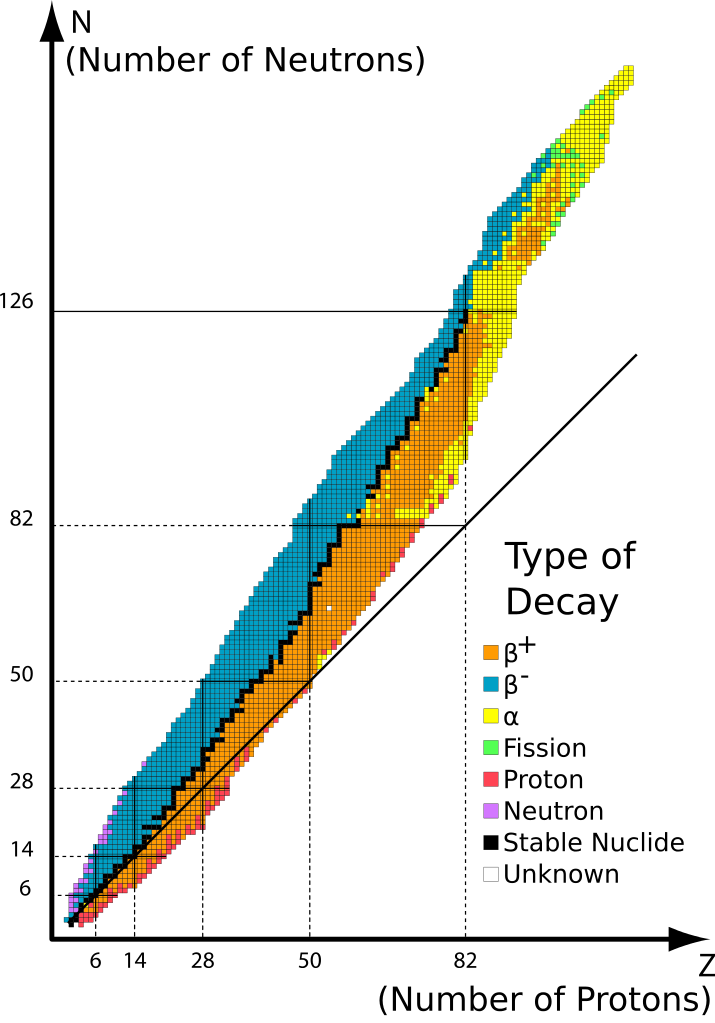
\includegraphics[width=0.9\textwidth]{images/line-nuclear-stability.png}
        \caption{Isotopes and their decay modes \cite{lineofnuclearstability}.}
        \label{fig:line of nuclear stability}
    \end{figure}
    
    \Cref{fig:line of nuclear stability} shows information on the decay of various nuclei as a function of their atomic number and neutron number.
    In particular the black nuclei are stable.
    There are 262 stable nuclei but it is theorised that approximately 7000 isotopes exist, most unstable.
    We have observed about 2000 of them.
    
    Up to about \(Z = 20\) we see that the stable nuclei have approximately \(N = Z\).
    After this the ratio of neutrons to protons gradually increases.
    This cannot be understood with the liquid drop model.
    This simplistic model would predict that \(Z = 0\) would form the most stable nuclei since this minimises the repulsive Coulomb force.
    The missing ingredient is quantum mechanics, in particular the Pauli exclusion principle.
    Protons and neutrons are both fermions, specifically they are spin \(1/2\) particles, and as such must obey the exclusion principle.
    A nucleus entirely made of neutrons would therefore have neutrons in much higher energy states than one with protons since protons and neutrons are distinguishable and so only need to satisfy the exclusion principle individually.
    
    The highest occupied energy level is the Fermi energy, \(\fermiEnergy\).
    It can be estimated by approximating the nucleus as a Fermi gas of freely moving fermions in a fixed volume, \(V\).
    If we consider only neutrons it can be shown that this treatment produces a density of
    \begin{equation}
        \frac{N}{V} = \frac{1}{3\pi^2} \left( \frac{2m_n\fermiEnergy}{2\hbar^2} \right)^{3/2}.
    \end{equation}
    
    Recall that the density of nuclear matter is approximately \(A/V \approx \rho_0 \approx 0.17\) nucleons per fermi cubed.
    For \(N = Z\) nuclei we then have \(N/V \approx 0.085\) neutrons per fermi cubed.
    This gives \(\fermiEnergy \approx \qty{38}{\MeV}\).
    This means that even the most energetic neutrons move relatively slowly and are therefore non-relativistic.
    
    The minimum energy required to remove a single neutron from the nucleus is the \defineindex{neutron separation energy}, \(S_\Pn\).
    This is defined as
    \begin{equation}
        S_{\Pn}(N, Z) = [M(N - 1, Z) + m_\Pn - M(N, Z)]c^2,
    \end{equation}
    or in terms of binding energies
    \begin{equation}
        S_{\Pn}(N, Z) = B(N, Z) - B(N - 1, Z).
    \end{equation}
    Since \(B(N, Z)/A \approx \qty{8}{\MeV}\) this implies a potential well depth of approximately \(S_\Pn + \fermiEnergy \approx \qty{46}{\MeV}\) for neutrons.
    
    For protons the result is a more shallow well due to the repulsive Coulomb force.
    This explains why for heavier nuclei we have \(N > Z\) for stable configurations.
    
    \section{Pairing Stability}
    There are four stable nuclei with both \(N\) and \(Z\) odd, they are \Pdeuteron, \ce{^6_3Li}, \ce{^10_5B}, and \ce{^14_7N}.
    There are 167 stable isotopes with both \(N\) and \(Z\) even.
    The reason for this is spin.
    While nucleons cannot have identical wave functions due to the exclusion principle the maximum overlap of wave functions, and hence maximum binding, occurs when the nucleons pair up into opposite spin pairs.
    
    The total angular momentum of a nucleon is
    \begin{equation}
        \vv{j} = \vv{l} + \vv{s}
    \end{equation}
    where \(\vv{l}\) and \(\vv{s}\) are the orbital angular momentum and the spin.
    When there is an even number of nucleons they can pair up with angular momenta \(+j\) and \(-j\).
    The effect is that the spin of the nucleus in the ground state for these even-even nuclei is \(j = 0\).
    
    For nuclei where \(A\) is odd, so either \(N\) or \(Z\) is odd, the spins still pair up leaving one nucleon unpaired, this will be the nucleon in the Fermi level.
    The spin of the nucleus is then the spin of this unpaired nucleon.
    
    \section{Nuclear Shell Model}
    When \(N = 2, 8, 20, 28, 50, 82, 126\), or \(Z = 2, 8, 20, 28, 50, 82\) nuclei were particularly stable.
    We call these \define{magic numbers}\index{magic number}.
    The explanation for this is that nuclei form a shell structure, much like electron shells in atomic physics.
    In order to derive this result we can treat the nuclei as moving independently in a potential well created by averaging out the short range nucleon-nucleon interactions.
    This takes a similar form to the nucleon density:
    \begin{equation}
        V(r) = -\frac{V_0}{1 + \exp[\frac{r - R}{a}]}.
    \end{equation}
    This is called the \defineindex{Woods--Saxon potential}.
    It looks like a square well with rounded corners.
    Since nucleons are typically non-relativistic we can treat the Woods-Saxon potential with the Schr\"odinger equation to predict the quantised energy levels.
    
    \begin{figure}
        \tikzsetnextfilename{woods-saxon}
        \begin{tikzpicture}
            \begin{axis}[
                width = 0.8\textwidth,
                xlabel = \(x\),
                ylabel = \(V(x)\),
                no markers,
                ytick = {0, -1},
                yticklabels = {0, \(-V_0\)},
                xtick = {-2, 0, 2},
                xticklabels = {-\(R\), 0, \(R\)},
                legend style={
                    at = {(0.5, 0.98)},
                    anchor = north,
                    draw = none
                },
                legend cell align = left
                ]
                \addplot[domain=0:4, highlight, very thick, samples=1000] (\x, {-1 / (1 + exp(100*(\x - 2)))});
                \addplot[domain=-4:0, highlight, very thick, samples=1000] (\x, {-1 / (1 + exp(100*(-\x - 2)))});
                \addplot[domain=0:4, tetrad blue, very thick, samples=1000] (\x, {-1 / (1 + exp(10*(\x - 2)))});
                \addplot[domain=-4:0, tetrad blue, very thick, samples=1000] (\x, {-1 / (1 + exp(10*(-\x - 2)))});
                \addplot[domain=0:4, tetrad purple, very thick, samples=1000] (\x, {-1 / (1 + exp(5*(\x - 2)))});
                \addplot[domain=-4:0, tetrad purple, very thick, samples=1000] (\x, {-1 / (1 + exp(5*(-\x - 2)))});
                \addplot[domain=0:4, tetrad green, very thick, samples=1000] (\x, {-1 / (1 + exp(2*(\x - 2)))});
                \addplot[domain=-4:0, tetrad green, very thick, samples=1000] (\x, {-1 / (1 + exp(2*(-\x - 2)))});
                \legend{\(a = 1/100\),,\(a = 1/10\),,\(a=1/5\),,\(a=1/2\)}
            \end{axis}
        \end{tikzpicture}
        \caption[Woods--Saxon potential.]{Woods--Saxon potential in one dimension. The parameter \(R\) controls the width of the potential well, \(a\) controls the steepness of the walls, and \(V_0\) controls the depth.}
    \end{figure}
    
    This alone doesn't quite predict the measured magic numbers.
    To match these we need to include in the potential a term known as \defineindex{spin-orbit coupling}, which describes the interaction between the spin and the orbital angular momentum.
    It is another central potential proportional to \(\vv{l}\cdot\vv{s}\), for a total potential
    \begin{equation}
        V = V(r) + V_{\mathrm{so}}(r)\vv{l}\cdot\vv{s}.
    \end{equation}
    This spin-orbit term is due to the strong force, not the electromagnetic force, and therefore has a large effect on the predictions compared to the same effect in the atomic structure, which is electromagnetic in origin.
    We can find \(\vv{l}\cdot\vv{s}\) by considering \(\vv{j}^2\):
    \begin{equation}
        \vv{j}^2 = \vv{l}^2 + \vv{s}^2 + 2\vv{l}\cdot\vv{s} \implies \vv{l}\cdot\vv{s} = \frac{1}{2}(\vv{j}^2 - \vv{l}^2 - \vv{s}^2).
    \end{equation}
    Now considering the action of the squared angular momentum operators on an eigenstate, \(\ket{l, s}\), we get eigenvalues \(j(j+1)\hbar^2\), and similar for \(\vv{l}\) and \(\vv{s}\).
    We conclude that
    \begin{equation}
        \vv{l}\cdot\vv{s} = [j(j + 1) - l(l + 1) - s(s + 1)]\frac{\hbar^2}{2}.
    \end{equation}
    
    The result of the \(\vv{l}\cdot\vv{s}\) term is splitting between energy levels with \(j = l \pm 1/2\).
    For \(s = 1/2\) we have \(j = l + 1/2\) so
    \begin{equation}
        \vv{l}\cdot\vv{s} = \frac{l\hbar^2}{2}
    \end{equation}
    and for \(s = -1/2\) the total angular momentum is \(j = l - 1/2\) and we have
    \begin{equation}
        \vv{l}\cdot\vv{s} = -\frac{1}{2}(l + 1)\hbar^2.
    \end{equation}
    The magnitude of the energy spitting caused by the spin-orbit term is then proportional to
    \begin{equation}
        \frac{1}{2}(2l + 1)\hbar^2.
    \end{equation}
    Note that higher values of \(j\) are more tightly bound since we consider binding energies to be positive.
    
    The energy levels as computed with increasingly accurate models are shown in \cref{fig:energy levels}.
    
    \begin{figure}
        \tikzsetnextfilename{energy-levels}
        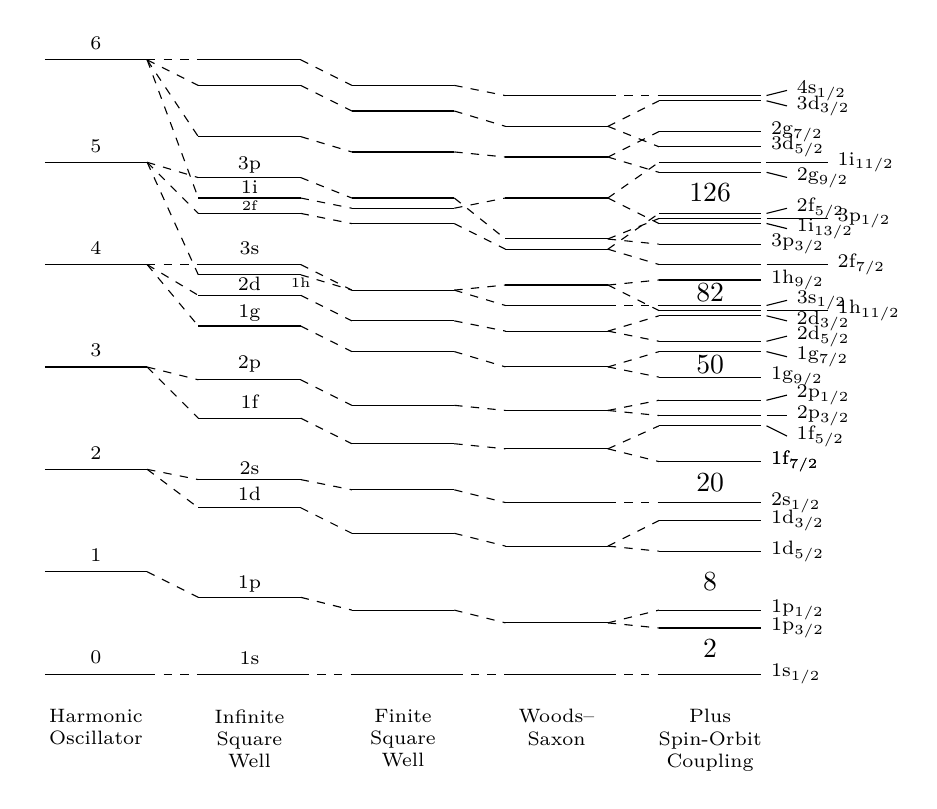
\begin{tikzpicture}[scale=0.65]
            \foreach \i in {0, ..., 6} {
                \coordinate (\i) at (0, 2*\i);
            }
            
            \node[below, font=\scriptsize] at (1, -0.5) {\parbox{1.5cm}{\centering Harmonic\\Oscillator}};
            \node[below, font=\scriptsize] at (4, -0.5) {\parbox{1.75cm}{\centering Infinite Square\\Well}};
            \node[below, font=\scriptsize] at (7, -0.5) {\parbox{1.5cm}{\centering Finite Square\\Well}};
            \node[below, font=\scriptsize] at (10, -0.5) {\parbox{1.5cm}{\centering Woods--Saxon}};
            \node[below, font=\scriptsize] at (13, -0.5) {\parbox{1.75cm}{\centering Plus Spin-Orbit\\Coupling}};
            
            % 0
            \coordinate (current pos) at (0);
            \foreach \y in {0, 0, 0, 0} {
                \draw (current pos) -- ++ (2, 0) coordinate (current pos);
                \draw[dashed] (current pos) -- ++ (1, \y) coordinate (current pos);
            }
            \draw (current pos) -- ++ (2, 0) coordinate (1s1);
            
            % 1
            \coordinate (current pos) at (1);
            \foreach \y in {-0.5, -0.25, -0.25, -0.1} {
                \draw (current pos) -- ++ (2, 0) coordinate (current pos);
                \draw[dashed] (current pos) -- ++ (1, \y) coordinate (current pos);
            }
            \draw (current pos) -- ++ (2, 0) coordinate (1p3);
            \draw[dashed] (11, 1) -- ++ (1, 0.25) coordinate (current pos);
            \draw (current pos) -- ++ (2, 0) coordinate (1p1);
            
            % 2
            \coordinate (current pos) at (2);
            \foreach \y in {-0.75, -0.5, -0.25, -0.1} {
                \draw (current pos) -- ++ (2, 0) coordinate (current pos);
                \draw[dashed] (current pos) -- ++ (1, \y) coordinate (current pos);
            }
            \draw (current pos) -- ++ (2, 0) coordinate (1d5);
            
            \coordinate (current pos) at (11, 2.5);
            \draw[dashed] (current pos) -- ++ (1, 0.5) coordinate (current pos);
            \draw (current pos) -- ++ (2, 0) coordinate (1d3);
            
            \coordinate (current pos) at ($(2) + (2, 0)$);
            \draw[dashed] (current pos) -- ++ (1, -0.2) coordinate (current pos);
            \foreach \y in {-0.2, -0.25, 0} {
                \draw (current pos) -- ++ (2, 0) coordinate (current pos);
                \draw[dashed] (current pos) -- ++ (1, \y) coordinate (current pos);
            }
            \draw (current pos) -- ++ (2, 0) coordinate (2s1);
            
            % 3
            \coordinate (current pos) at (3);
            \foreach \y in {-1, -0.5, -0.1, -0.25} {
                \draw (current pos) -- ++ (2, 0) coordinate (current pos);
                \draw[dashed] (current pos) -- ++ (1, \y) coordinate (current pos);
            }
            \draw (current pos) -- ++ (2, 0) coordinate (1f7);
            
            \coordinate (current pos) at (11, 4.4);
            \draw[dashed] (current pos) -- ++ (1, 0.45) coordinate (current pos);
            \draw (current pos) -- ++ (2, 0) coordinate (1f5);
            
            \coordinate (current pos) at ($(3) + (2, 0)$);
            \draw[dashed] (current pos) -- ++ (1, -0.25) coordinate (current pos);
            \foreach \y in {-0.5, -0.1, -0.1} {
                \draw (current pos) -- ++ (2, 0) coordinate (current pos);
                \draw[dashed] (current pos) -- ++ (1, \y) coordinate (current pos);
            }
            \draw (current pos) -- ++ (2, 0) coordinate (2p3);
            
            \coordinate (current pos) at (11, 5.15);
            \draw[dashed] (current pos) -- ++ (1, 0.2) coordinate (current pos);
            \draw (current pos) -- ++ (2, 0) coordinate (2p1);
            
            % 4
            \coordinate (current pos) at (4);
            \foreach \y in {-1.2, -0.5, -0.3, -0.2} {
                \draw (current pos) -- ++ (2, 0) coordinate (current pos);
                \draw[dashed] (current pos) -- ++ (1, \y) coordinate (current pos);
            }
            \draw (current pos) -- ++ (2, 0) coordinate (1g9);
            
            \coordinate (current pos) at (11, 6);
            \draw[dashed] (current pos) -- ++ (1, 0.3) coordinate (current pos);
            \draw (current pos) -- ++ (2, 0) coordinate (1g7);
            
            \coordinate (current pos) at ($(4) + (2, 0)$);
            \draw[dashed] (current pos) -- ++ (1, -0.6) coordinate (current pos);
            \foreach \y in {-0.5, -0.2, -0.2} {
                \draw (current pos) -- ++ (2, 0) coordinate (current pos);
                \draw[dashed] (current pos) -- ++ (1, \y) coordinate (current pos);
            }
            \draw (current pos) -- ++ (2, 0) coordinate (2d5);
            
            \coordinate (current pos) at ($(4) + (2, 0)$);
            \draw[dashed] (current pos) -- ++ (1, 0) coordinate (current pos);
            \foreach \y in {-0.5, -0.3, 0} {
                \draw (current pos) -- ++ (2, 0) coordinate (current pos);
                \draw[dashed] (current pos) -- ++ (1, \y) coordinate (current pos);
            }
            \draw (current pos) -- ++ (2, 0) coordinate (3s1);
            
            \coordinate (current pos) at (11, 6.7);
            \draw[dashed] (current pos) -- ++ (1, 0.3) coordinate (current pos);
            \draw (current pos) -- ++ (2, 0) coordinate (2d3);
            
            % 5
            \coordinate (current pos) at (5);
            \foreach \y in {-2.2, -0.3, 0.1, -0.5} {
                \draw (current pos) -- ++ (2, 0) coordinate (current pos);
                \draw[dashed] (current pos) -- ++ (1, \y) coordinate (current pos);
            }
            \draw (current pos) -- ++ (2, 0) coordinate (1h11);
            
            \coordinate (current pos) at ($(5) + (2, 0)$);
            \draw[dashed] (current pos) -- ++ (1, -1) coordinate (current pos);
            \foreach \y in {-0.2, -0.5, -0.3} {
                \draw (current pos) -- ++ (2, 0) coordinate (current pos);
                \draw[dashed] (current pos) -- ++ (1, \y) coordinate (current pos);
            }
            \draw (current pos) -- ++ (2, 0) coordinate (2f7);
            
            \coordinate (current pos) at (11, 8.3);
            \draw[dashed] (current pos) -- ++ (1, 0.7) coordinate (current pos);
            \draw (current pos) -- ++ (2, 0) coordinate (2f5);
            
            \coordinate (current pos) at ($(5) + (2, 0)$);
            \draw[dashed] (current pos) -- ++ (1, -0.3) coordinate (current pos);
            \foreach \y in {-0.4, -0.8, 0.4} {
                \draw (current pos) -- ++ (2, 0) coordinate (current pos);
                \draw[dashed] (current pos) -- ++ (1, \y) coordinate (current pos);
            }
            \draw (current pos) -- ++ (2, 0) coordinate (3p1);
            
            \coordinate (current pos) at (11, 8.5);
            \draw[dashed] (current pos) -- ++ (1, -0.1) coordinate (current pos);
            \draw (current pos) -- ++ (2, 0) coordinate (3p3);
            
            \coordinate (current pos) at (11, 7.6);
            \draw [dashed] (current pos) -- ++ (1, 0.1) coordinate (current pos);
            \draw (current pos) -- ++ (2, 0) coordinate (1h9);
            
            % 6
            \coordinate (current pos) at (6);
            \foreach \y in {-2.7, -0.2, 0.2, -0.5} {
                \draw (current pos) -- ++ (2, 0) coordinate (current pos);
                \draw[dashed] (current pos) -- ++ (1, \y) coordinate (current pos);
            }
            \draw (current pos) -- ++ (2, 0) coordinate (1i13);
            
            \coordinate (current pos) at (11, 9.3);
            \draw[dashed] (current pos) -- ++ (1, 0.7) coordinate (current pos);
            \draw (current pos) -- ++ (2, 0) coordinate (1i11);
            
            \coordinate (current pos) at ($(6) + (2, 0)$);
            \draw[dashed] (current pos) -- ++ (1, -1.5) coordinate (current pos);
            \foreach \y in {-0.3, -0.1, -0.3} {
                \draw (current pos) -- ++ (2, 0) coordinate (current pos);
                \draw[dashed] (current pos) -- ++ (1, \y) coordinate (current pos);
            }
            \draw (current pos) -- ++ (2, 0) coordinate (2g9);
            
            \coordinate (current pos) at (11, 10.1);
            \draw[dashed] (current pos) -- ++ (1, 0.5) coordinate (current pos);
            \draw (current pos) -- ++ (2, 0) coordinate (2g7);
            
            \coordinate (current pos) at ($(6) + (2, 0)$);
            \draw[dashed] (current pos) -- ++ (1, -0.5) coordinate (current pos);
            \foreach \y in {-0.5, -0.3, -0.4} {
                \draw (current pos) -- ++ (2, 0) coordinate (current pos);
                \draw[dashed] (current pos) -- ++ (1, \y) coordinate (current pos);
            }
            \draw (current pos) -- ++ (2, 0) coordinate (3d5);
            
            \coordinate (current pos) at (11, 10.7);
            \draw[dashed] (current pos) -- ++ (1, 0.5) coordinate (current pos);
            \draw (current pos) -- ++ (2, 0) coordinate (3d3);
            
            \coordinate (current pos) at ($(6) + (2, 0)$);
            \draw[dashed] (current pos) -- ++ (1, 0) coordinate (current pos);
            \foreach \y in {-0.5, -0.2, 0} {
                \draw (current pos) -- ++ (2, 0) coordinate (current pos);
                \draw[dashed] (current pos) -- ++ (1, \y) coordinate (current pos);
            }
            \draw (current pos) -- ++ (2, 0) coordinate (4s1);
            
            
            % State labels
            \node[right, font=\scriptsize] at (1s1) {1s\textsubscript{1/2}};
            \node[right, font=\scriptsize] at (1p3) {1p\textsubscript{3/2}};
            \node[right, font=\scriptsize] at (1p1) {1p\textsubscript{1/2}};
            \node[right, font=\scriptsize] at (1d5) {1d\textsubscript{5/2}};
            \node[right, font=\scriptsize] at (1d3) {1d\textsubscript{3/2}};
            \node[right, font=\scriptsize] at (2s1) {2s\textsubscript{1/2}};
            \node[right, font=\scriptsize] at (1f7) {1f\textsubscript{7/2}};
            \draw ($(1f5) + (0.1, 0)$) -- ($(1f5) + (0.5, -0.2)$) node[right, font=\scriptsize] {1f\textsubscript{5/2}};
            \draw ($(2p3) + (0.1, 0)$) -- ($(2p3) + (0.5, 0)$) node[right, font=\scriptsize] {2p\textsubscript{3/2}};
            \draw ($(2p1) + (0.1, 0)$) -- ($(2p1) + (0.5, 0.1)$) node[right, font=\scriptsize] {2p\textsubscript{1/2}};
            \node[right, font=\scriptsize] at (1g9) {1g\textsubscript{9/2}};
            \draw ($(1g7) + (0.1, 0)$) -- ($(1g7) + (0.5, -0.1)$) node[right, font=\scriptsize] {1g\textsubscript{7/2}};
            \draw ($(2d5) + (0.1, 0)$) -- ($(2d5) + (0.5, 0.1)$) node[right, font=\scriptsize] {2d\textsubscript{5/2}};
            \draw ($(2d3) + (0.1, 0)$) -- ($(2d3) + (0.5, -0.1)$) node[right, font=\scriptsize] {2d\textsubscript{3/2}};
            \draw ($(1h11) + (0.1, 0)$) -- ($(1h11) + (1.3, 0)$) node[right, font=\scriptsize] {1h\textsubscript{11/2}};
            \draw ($(3s1) + (0.1, 0)$) -- ($(3s1) + (0.5, 0.1)$) node[right, font=\scriptsize] {3s\textsubscript{1/2}};
            \node[right, font=\scriptsize] at (1f7) {1f\textsubscript{7/2}};
            \node[right, font=\scriptsize] at (1h9) {1h\textsubscript{9/2}};
            \draw ($(2f7) + (0.1, 0)$) -- ($(2f7) + (1.3, 0)$) node[right, font=\scriptsize] {2f\textsubscript{7/2}};
            \draw ($(3p1) + (0.1, 0)$) -- ($(3p1) + (1.3, 0)$) node[right, font=\scriptsize] {3p\textsubscript{1/2}};
            \draw ($(2f5) + (0.1, 0)$) -- ($(2f5) + (0.5, 0.1)$) node[right, font=\scriptsize] {2f\textsubscript{5/2}};
            \node[right, font=\scriptsize] at (3p3) {3p\textsubscript{3/2}};
            \draw ($(1i13) + (0.1, 0)$) -- ($(1i13) + (0.5, -0.1)$) node[right, font=\scriptsize] {1i\textsubscript{13/2}};
            \draw ($(1i11) + (0.1, 0)$) -- ($(1i11) + (1.3, 0)$) node[right, font=\scriptsize] {1i\textsubscript{11/2}};
            \draw ($(2g9) + (0.1, 0)$) -- ($(2g9) + (0.5, -0.1)$) node[right, font=\scriptsize] {2g\textsubscript{9/2}};
            \node[right, font=\scriptsize] at (2g7) {2g\textsubscript{7/2}};
            \node[right, font=\scriptsize] at (3d5) {3d\textsubscript{5/2}};
            \draw ($(3d3) + (0.1, 0)$) -- ($(3d3) + (0.5, -0.1)$) node[right, font=\scriptsize] {3d\textsubscript{3/2}};
            \draw ($(4s1) + (0.1, 0)$) -- ($(4s1) + (0.5, 0.1)$) node[right, font=\scriptsize] {4s\textsubscript{1/2}};
            
            % Magic numbers
            \node at (13, 0.5) {2};
            \node at (13, 1.8) {8};
            \node at (13, 3.75) {20};
            \node at (13, 6.05) {50};
            \node at (13, 7.45) {82};
            \node at (13, 9.4) {126};
            
            % Principle Quantum numbers
            \foreach \i in {0, ..., 6} {
                \node[above, font=\scriptsize] at (1, 2*\i) {\i};
            }
            
            % Angular momentum
            \node[above, font=\scriptsize] at (4, 0) {1s};
            \node[above, font=\scriptsize] at (4, 1.4) {1p};
            \node[above, font=\scriptsize] at (4, 3.2) {1d};
            \node[above, font=\scriptsize] at (4, 3.7) {2s};
            \node[above, font=\scriptsize] at (4, 5) {1f};
            \node[above, font=\scriptsize] at (4, 5.7) {2p};
            \node[above, font=\scriptsize] at (4, 6.7) {1g};
            \node[above, font=\scriptsize] at (4, 7.3) {2d};
            \node[font=\tiny] at (5, 7.65) {1h};
            \node[above, font=\scriptsize] at (4, 8) {3s};
            \node[above, font=\tiny] at (4, 8.86) {2f};
            \node[above, font=\scriptsize] at (4, 9.2) {1i};
            \node[above, font=\scriptsize] at (4, 9.6) {3p};
        \end{tikzpicture}
        \caption[Energy levels in various models.]{Nuclear energy levels as calculated from increasingly accurate models. The simplest being the evenly spaced energy levels of the harmonic oscillator, then an infinite square well, these energies are then reduced slightly by considering a finite square well, another improvement comes from considering the Woods--Saxon potential, which is a square well with rounded edges, and a final improvement by including a spin-orbit coupling term. The numbers above the final energy levels are the magic numbers.}
        \label{fig:energy levels}
    \end{figure}
    
    \subsection{Nuclear Subshells}
    We can specify a subshell with the notation \(nl_j\) where \(n\) is a positive integer where \(nl_j\) is higher energy than \(ml_j\) if \(n > m\), \(l\) corresponds to the orbital angular momentum of the subshell, and \(j\) to the total angular momentum.
    For example, \(2\mathrm{d}_{3/2}\) corresponds to the second lowest level (\(n = 2\)), with orbital angular momentum \(l = 2\) (\(\mathrm{d}\) corresponds to the second state (\(\mathrm{s}\), \(\mathrm{p}\), \(\mathrm{d}\), \(\mathrm{f}\) \dots correspond to 0, 1, 2, 3, \dots)) and total angular momentum \(j = 3/2\).
    
    \(n\) corresponds to the number of nodes of the wave function, that is points where the wave function is zero, excluding nodes at infinity (since we assume wave functions vanish at infinity).
    Higher values of \(l\) correspond to the first maximum of the wave function being further from the origin, which is what one would naively expect from a high angular momentum state.
    Unlike in atomic physics any value of \(l\) can go with any value of \(n\).
    
    Each subshell has \((2j + 1)\)-fold degeneracy, corresponding to the magnetic sub-states \(m_{j} = -j, \dotsc, j\).
    For example, for \(2\mathrm{d}_{3/2}\) there are \(2(3/2) + 1 = 4\) magnetic sub-states, \(m_j = -3/2, -1/2, 1/2, 3/2\).
    This means that a maximum of four protons or four neutrons can be in this subshell.
    
    A major shell consists of a selection of subshells separated by a larger than normal gap.
    When a major shell is full the nucleus is particularly stable.
    We call nucleon numbers resulting in full shells \define{magic numbers}\index{magic number}.
    The first few magic numbers are 2, 8, 20, 28, 28, 50, 82, and 126.
    Since protons and neutrons have separate shell structures it is possible that both the proton number and neutron number can be magic, in which case we say the nucleus is \defineindex{doubly magic}, and these are some of the most stable nuclei.
    
    \begin{figure}
        \tikzsetnextfilename{oxygen-energy-levels}
        \begin{tikzpicture}
            \draw (0, 0) -- (2, 0);
            \draw (0, 2) -- (2, 2);
            \draw (0, 3) -- (2, 3);
            \draw (0, 5) -- (2, 5);
            
            \fill[highlight] (0.5, 0) circle [radius = 0.1cm];
            \fill[highlight] (1.5, 0) circle [radius = 0.1cm];
            \fill[highlight] (0.25, 2) circle [radius = 0.1cm];
            \fill[highlight] (0.75, 2) circle [radius = 0.1cm];
            \fill[highlight] (1.25, 2) circle [radius = 0.1cm];
            \fill[highlight] (1.75, 2) circle [radius = 0.1cm];
            \fill[highlight] (0.5, 0) circle [radius = 0.1cm];
            \fill[highlight] (1.5, 0) circle [radius = 0.1cm];
            \fill[highlight] (0.5, 3) circle [radius = 0.1cm];
            \fill[highlight] (1.5, 3) circle [radius = 0.1cm];
            \draw[highlight] (2/7, 5) circle [radius = 0.1cm];
            \draw[highlight] (4/7, 5) circle [radius = 0.1cm];
            \draw[highlight] (6/7, 5) circle [radius = 0.1cm];
            \draw[highlight] (8/7, 5) circle [radius = 0.1cm];
            \draw[highlight] (10/7, 5) circle [radius = 0.1cm];
            \draw[highlight] (12/7, 5) circle [radius = 0.1cm];
            
            \node[font=\scriptsize] at (1, -0.5) {\parbox{2cm}{\centering \ce{O} (\(Z = 8\))\\protons}};
            
            \node[left] at (0, 0) {\(1\mathrm{s}_{1/2}\)};
            \node[left] at (0, 2) {\(1\mathrm{p}_{3/2}\)};
            \node[left] at (0, 3) {\(1\mathrm{p}_{1/2}\)};
            \node[left] at (0, 5) {\(1\mathrm{d}_{5/2}\)};
            
            \begin{scope}[xshift=3cm]
                \draw (0, 0) -- (2, 0);
                \draw (0, 2) -- (2, 2);
                \draw (0, 3) -- (2, 3);
                \draw (0, 5) -- (2, 5);
                
                \fill[highlight] (0.5, 0) circle [radius = 0.1cm];
                \fill[highlight] (1.5, 0) circle [radius = 0.1cm];
                \fill[highlight] (0.25, 2) circle [radius = 0.1cm];
                \fill[highlight] (0.75, 2) circle [radius = 0.1cm];
                \fill[highlight] (1.25, 2) circle [radius = 0.1cm];
                \fill[highlight] (1.75, 2) circle [radius = 0.1cm];
                \fill[highlight] (0.5, 0) circle [radius = 0.1cm];
                \fill[highlight] (1.5, 0) circle [radius = 0.1cm];
                \fill[highlight] (0.5, 3) circle [radius = 0.1cm];
                \draw[highlight] (1.5, 3) circle [radius = 0.1cm];
                \draw[highlight] (2/7, 5) circle [radius = 0.1cm];
                \draw[highlight] (4/7, 5) circle [radius = 0.1cm];
                \draw[highlight] (6/7, 5) circle [radius = 0.1cm];
                \draw[highlight] (8/7, 5) circle [radius = 0.1cm];
                \draw[highlight] (10/7, 5) circle [radius = 0.1cm];
                \draw[highlight] (12/7, 5) circle [radius = 0.1cm];
                
                \node[font=\scriptsize] at (1, -0.5) {\parbox{2cm}{\centering \ce{^15O} (\(N = 7\))\\neutrons}};
            \end{scope}
            \begin{scope}[xshift=6cm]
                \draw (0, 0) -- (2, 0);
                \draw (0, 2) -- (2, 2);
                \draw (0, 3) -- (2, 3);
                \draw (0, 5) -- (2, 5);
                
                \fill[highlight] (0.5, 0) circle [radius = 0.1cm];
                \fill[highlight] (1.5, 0) circle [radius = 0.1cm];
                \fill[highlight] (0.25, 2) circle [radius = 0.1cm];
                \fill[highlight] (0.75, 2) circle [radius = 0.1cm];
                \fill[highlight] (1.25, 2) circle [radius = 0.1cm];
                \fill[highlight] (1.75, 2) circle [radius = 0.1cm];
                \fill[highlight] (0.5, 0) circle [radius = 0.1cm];
                \fill[highlight] (1.5, 0) circle [radius = 0.1cm];
                \fill[highlight] (0.5, 3) circle [radius = 0.1cm];
                \fill[highlight] (1.5, 3) circle [radius = 0.1cm];
                \draw[highlight] (2/7, 5) circle [radius = 0.1cm];
                \draw[highlight] (4/7, 5) circle [radius = 0.1cm];
                \draw[highlight] (6/7, 5) circle [radius = 0.1cm];
                \draw[highlight] (8/7, 5) circle [radius = 0.1cm];
                \draw[highlight] (10/7, 5) circle [radius = 0.1cm];
                \draw[highlight] (12/7, 5) circle [radius = 0.1cm];
                
                \node[font=\scriptsize] at (1, -0.5) {\parbox{2cm}{\centering \ce{^16O} (\(N = 8\))\\neutrons}};
            \end{scope}
            \begin{scope}[xshift=9cm]
                \draw (0, 0) -- (2, 0);
                \draw (0, 2) -- (2, 2);
                \draw (0, 3) -- (2, 3);
                \draw (0, 5) -- (2, 5);
                
                \fill[highlight] (0.5, 0) circle [radius = 0.1cm];
                \fill[highlight] (1.5, 0) circle [radius = 0.1cm];
                \fill[highlight] (0.25, 2) circle [radius = 0.1cm];
                \fill[highlight] (0.75, 2) circle [radius = 0.1cm];
                \fill[highlight] (1.25, 2) circle [radius = 0.1cm];
                \fill[highlight] (1.75, 2) circle [radius = 0.1cm];
                \fill[highlight] (0.5, 0) circle [radius = 0.1cm];
                \fill[highlight] (1.5, 0) circle [radius = 0.1cm];
                \fill[highlight] (0.5, 3) circle [radius = 0.1cm];
                \fill[highlight] (1.5, 3) circle [radius = 0.1cm];
                \fill[highlight] (2/7, 5) circle [radius = 0.1cm];
                \draw[highlight] (4/7, 5) circle [radius = 0.1cm];
                \draw[highlight] (6/7, 5) circle [radius = 0.1cm];
                \draw[highlight] (8/7, 5) circle [radius = 0.1cm];
                \draw[highlight] (10/7, 5) circle [radius = 0.1cm];
                \draw[highlight] (12/7, 5) circle [radius = 0.1cm];
                
                \node[font=\scriptsize] at (1, -0.5) {\parbox{2cm}{\centering \ce{^17O} (\(N = 9\))\\neutrons}};
            \end{scope}
        \end{tikzpicture}
        \caption[Energy levels of oxygen nuclei.]{Energy levels for three isotopes of oxygen, the proton energy levels are the same for all three, they differ only in the number of neutrons. \tikzexternaldisable \protect\tikz{\fill[highlight] (0, 0) circle[radius=0.1cm]} represents a filled energy level and \protect\tikz{\draw[highlight] (0, 0) circle[radius=0.1cm]} represents an empty energy level.\tikzexternalenable}
        \label{fig:oxygen energy levels}
    \end{figure}
    
    For example, \ce{^16O} has 8 protons and 8 neutrons, so is doubly magic.
    It is therefore significantly more stable than \ce{^15O} and \ce{^17O}.
    In fact, \ce{^15O} isn't even stable, it decays into \ce{^15N} by \APbeta{} decay.
    \ce{^16O} makes up \qty{99.76}{\percent} of all oxygen isotopes, \ce{^17O} makes up only \qty{0.038}{\percent} of oxygen.
    Oxygen \ce{^18O} is slightly more stable making up \qty{0.205}{\percent} of oxygen, the slight increase in stability is due to the effect of spin pairing, in which opposite spin nucleons pair up to give net-zero spin.
    In general even-even nuclei are slightly more stable than nearby odd-even, or odd-odd nuclei.
    The energy levels for oxygen are shown in \cref{fig:oxygen energy levels}.
    
    \subsection{Parity}
    We define the parity operator, \(P\), as having the action \(P\psi(\vv{r}) = \psi(-\vv{r})\).
    The \defineindex{parity} of a state is then the eigenvalue of the parity operator, an even parity state has eigenvalue \(+1\), meaning \(\psi(-\vv{r}) = \psi(\vv{r})\), and an odd parity state has eigenvalue \(-1\), meaning \(\psi(-\vv{r}) = -\psi(\vv{r})\).
    The parity of a subshell is controlled by the unpaired nucleon, if there is one, since it can be shown that the parity is \((-1)^{l}\).
    Notice that this means all even-even states have even parity.
    
    \chapter{Excited States of Nuclei}
    So far we have considered nuclei in their ground state.
    Nuclei can also have excited, higher energy states.
    Taking the earlier example of \ce{^17O} (see \cref{fig:oxygen energy levels}) its first excited state consists of promoting one of the \(1\mathrm{p}_{1/2}\) neutrons to the \(1\mathrm{d}_{5/2}\) state.
    When this happens the promoted neutron pairs with the neutron already in this state.
    The overall parity and spin of the nucleus is then determined by the position of the hole left behind.
    
    We call two nuclei \defineindex{mirror nuclei} if the proton number of one is the neutron number of the other and vice versa.
    Such nuclei have similar energy excited states since the main energy contribution comes from the strong force, which acts the same between protons and neutrons.
    The energy levels aren't exactly the same however, as the coulomb force does contribute a bit.
    
    \section{Excited States of Even-Even Nuclei}
    Most even-even nuclei have a similar first excited state, which we refer to as a \(2^+\) state.
    Thinking of the shell model we would not expect excited states to be the same across nuclei as the excited state should depend on what the next available energy level is.
    The reason for these excited states being mostly the same is that it is not a single nucleon that becomes excited.
    Instead there is a collective excitation of all nucleons.
    
    In the liquid drop model we can think of this as the state vibrating around its spherical equilibrium.
    We refer to a single quanta of vibration as a \defineindex{phonon}.
    The first \(2^+\) state corresponds to a single phonon.
    See \cref{fig:nuclear deformation}.
    The next excitation for these nuclei is usually a \(4^+\) state, which corresponds to two \(2^+\) phonons coupling.
    The energy of the \(4^+\) state is then approximately double that of the \(2^+\) state.
    
    \begin{figure}
        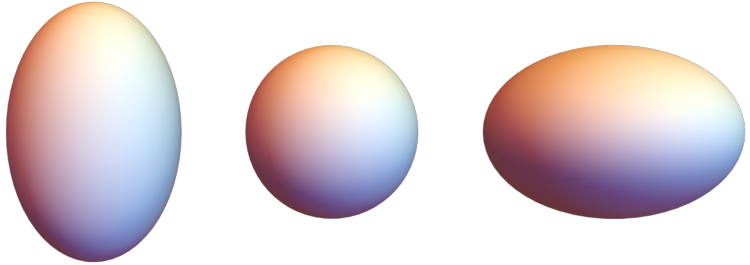
\includegraphics[width=0.8\textwidth]{images/nucleus-deformation.pdf}
        \caption[Nuclear deformation]{A nucleus oscillates around its equilibrium spherical shape. Oscillating from a prolate, rugby ball shape, to a flatter, oblate shape.}
        \label{fig:nuclear deformation}
    \end{figure}
    
    Many even-even nuclei with \(A > 150\) don't follow this pattern of doubling energy with each excitation.
    Instead we find that the excitation scales as \(j(j + 1)\).
    This dependence on the angular momentum suggests that the energy is associated with rotations of the nucleus, similar to excitation of diatomic molecules.
    This tells us something interesting about these nuclei.
    They must not be spherically symmetric since in quantum mechanics a spherical state doesn't change under rotations, and therefore has the same energy as before the rotation.
    These larger nuclei are therefore permanently deformed, usually to form a prolate, rugby ball, shape.
    
    If the ratio of major to minor axes exceeds \(2\colon1\) then we say the nucleus is superdeformed.
    Such states have been observed at very high spins, \(j \approx 60 \hbar\).
    
    The question then arises as to why permanently deformed states form.
    The liquid drop model fails to answer this question, it predicts that a spherical state is always most stable.
    We have to consider individual nucleon orbitals.
    Only wave functions corresponding to \(\mathrm{s}\)-states, which all have \(l = 0\), are spherically symmetric.
    The angular dependence of states enters through the spherical harmonics, \(Y_{lm}(\vartheta, \varphi)\), which are constant only when \(l = 0\).
    For deformed nuclei the asymmetric states split in energy depending on the value of \(m_j\).
    The size and sign of the split depends on the shape and size of the nuclear deformation.
    The exact maths demonstrating this is beyond the scope of the course but we can see why roughly with a few plots and some intuition.
    
    \begin{figure}
        \tikzsetnextfilename{mj-orbitals}
        \begin{tikzpicture}
            \draw[very thick, ->] (0, 0) -- (3, 0);
            
            \draw[highlight, ->, very thick] (0, 0) -- (80:3) node[pos=1.02, right, black] {\(m_j = 1/2\)};
            \draw[highlight!80, ->, very thick] (0, 0) -- (65:3) node[right, black] {\(m_j = 3/2\)};
            \draw[highlight!60, ->, very thick] (0, 0) -- (50:3) node[right, black] {\(m_j = 5/2\)};
            \draw[highlight!40, ->, very thick] (0, 0) -- (35:3) node[right, black] {\(m_j = 7/2\)};
            
            \draw[highlight] (80:3) -- (0, 0 -| 80:3);
            \draw[highlight!80] (65:3) -- (0, 0 -| 65:3);
            \draw[highlight!60] (50:3) -- (0, 0 -| 50:3);
            \draw[highlight!40] (35:3) -- (0, 0 -| 35:3);
            
            \draw[highlight, rotate=-10, very thick] (0, 0) circle [x radius = 1, y radius = 0.5];
            \draw[highlight!80, rotate=-25, very thick] (0, 0) circle [x radius = 1, y radius = 0.5];
            \draw[highlight!60, rotate=-40, very thick] (0, 0) circle [x radius = 1, y radius = 0.5];
            \draw[highlight!40, rotate=-55, very thick] (0, 0) circle [x radius = 1, y radius = 0.5];
        \end{tikzpicture}
        \caption{An intuitive picture of orbitals for different values of \(m_j\).}
        \label{fig:mj orbitals}
    \end{figure}
    
    Consider \cref{fig:mj orbitals}.
    We can think of the orbitals for different values of \(m_j\) as being circles perpendicular to the angular momentum.
    Notice that as \(m_j\) increases these start to overlap more with a state which is stretched in the vertical direction.
    This increases the stability of the state, and so for high angular momentum states, which allow large values of \(m_j\), deformed states are more stable.
    The same logic applies to states squashed in the vertical direction, we simply consider negative values of \(m_j\).
    
    This applies to each individual nucleon.
    If enough nucleons have a reduced single particle energy by forming deformed states then overall a deformed shape will be energetically favourable.
    
    \chapter{The Weak Force}
    \section{Beta Decay}
    Beta decay is mediated by the weak force.
    A free neutron will beta decay with a lifetime of approximately 15 minutes, the process is
    \begin{equation}
        \Pn \to \Pp + \Pe + \APnue.
    \end{equation}
    Here \APnue{} is an electron antineutrino, which is a neutral, fundamental particle with a small, but nonzero, mass, which is less than \qty[per-mode=symbol]{2}{\electronvolt\per\clight\squared}, and spin 1/2.
    A free proton cannot decay in this way (even swapping an electron for a positron for charge conservation) since \(m_{\Pp} < m_{\Pn}\).
    
    Beta decay is a weak process occurring on the quark level:
    \begin{equation}
        \tikzsetnextfilename{feynman-beta-decay}
        \begin{tikzpicture}[baseline=(current bounding box)]
            \begin{feynman}
                \vertex (d1 in) {\Pd};
                \vertex (d2 in) at (0, 0.5) {\Pd};
                \vertex (u1 in) at (0, 1) {\Pu};
                \vertex (u1 out) at (4, 1) {\Pu};
                \vertex (u2 out) at (4, 0) {\Pu};
                \vertex (d2 out) at (4, 0.5) {\Pd};
                \vertex (emit boson) at (1.5, 0);
                \vertex (boson decay) at (2.5, -0.75);
                \vertex (electron) at (4, -0.5) {\Pe};
                \vertex (neutrino) at (4, -1) {\APnue};
                \diagram {
                    (d1 in) -- [fermion] (emit boson) -- [fermion] (u2 out);
                    (d2 in) -- [fermion] (d2 out);
                    (u1 in) -- [fermion] (u1 out);
                    (emit boson) -- [boson, edge label'=\PWm] (boson decay) -- [fermion] (electron);
                    (boson decay) -- [anti fermion] (neutrino);
                };
            \end{feynman}
            \draw[decorate, decoration={brace, amplitude=5pt, mirror, raise=4pt}] (u1 in.north) -- (d1 in.south) node[left, midway, xshift=-2ex] {\Pn};
            \draw[decorate, decoration={brace, amplitude=5pt, raise=4pt}] (u1 out.north) -- (u2 out.south) node[right, midway, xshift=2ex] {\Pp};
        \end{tikzpicture}
    \end{equation}
    
    The range of the wake interaction, as with all interactions, depends on the mass of the exchange particle, which is a \PWpm{} or \PZzero.
    The mass of \PWpm{} is \(m_{\PW} = \qty[per-mode=symbol]{80.4}{\giga\electronvolt\per\clight\squared}\).
    This is very large, so the weak force has a very small range,
    \begin{equation}
        R_{\PW} = \frac{\hbar}{m_{\PW}c} = \frac{\hbar c}{m_{\PW}c^2} \approx \frac{\qty{197}{\mega\electronvolt\fermi}}{(\qty{80.4e3}{\MeVpercsquared})c^2} \approx \qty{2e-3}{\fermi}.
    \end{equation}
    
    \subsection{Beta Decay in the Nucleus}
    For nuclei with an excess of neutrons, relative to the line of stability, the beta decay process can convert a neutron into a proton, for example,
    \begin{equation}
        \ce{^19_8O} \to \ce{^19_9 F} + \Pe + \APnue.
    \end{equation}
    The beta minus process can occur energetically so long as
    \begin{equation}
        M(N, Z) > M(N - 1, Z + 1).
    \end{equation}
    That is the resulting nuclei must be lighter than the initial nuclei.
    Note that we are using neutral atomic masses, and so the extra atomic electron is already accounted for.
    We also neglect the mass of the neutrino since it is so small.
    
    For nuclei with an excess of protons, relative to the line of stability, the beta decay process can convert a proton into a neutron, for example,
    \begin{equation}
        \ce{^18_9F} \to \ce{^18_8O} + \APe + \Pnue.
    \end{equation}
    The beta plus decay process can occur energetically so long as
    \begin{equation}
        M(N, Z) > M(N + 1, Z - 1) + 2m_{\Peneutral}.
    \end{equation}
    Notice that we must consider the mass of the positron that is produced, as well as the extra electron on top of the atomic electrons.
    
    There is a second process by which a proton can be converted into a neutron in a nucleus, namely electron capture, in which an atomic electron combines with a proton to create a neutron, for example,
    \begin{equation}
        \ce{^7_4Be} + \Pe \to \ce{^7_3Li} + \Pnue.
    \end{equation}
    This only requires that
    \begin{equation}
        M(N, Z) > M(N + 1, Z - 1),
    \end{equation}
    since there is no left over electron or positron.
    
    For some nuclei beta plus decay is energetically forbidden but electron capture is not.
    However, many nuclei can, and do, decay by either mode.
    In general proton or neutron rich nuclei will decay by some combination of beta plus/minus decay and electron capture until they can no longer decay this way.
    Typically this renders them stable, although if they are massive enough there may be other decay modes.
    
    \subsection{Neutrinos}
    Some of the first evidence for neutrinos was in the energy spectrum of the electrons produced in beta decay.
    In a two particle decay we expect that the energy of decay products is fixed by the energy of the decaying particle, for example, we find this in electron capture.
    This is not what we find measuring the energy of electrons produced in beta decay.
    Instead we find a range of kinetic energies between zero and some upper maximum.
    This is evidence that there is some other particle produced in the decay, and the varying kinetic energy is due to the variety of ways of sharing kinetic energy between the particles produced.
    
    \section{Thermonuclear Fusion}
    As well as beta decay the weak force is also involved in the power generation in the sun.
    The first nuclear reaction to occur in a star is
    \begin{equation}
        2\Pp \to \Pdeuteron + \APe + \Pnue.
    \end{equation}
    This is a weak interaction process, since one of the protons becomes a neutron.
    Because of this it is much slower than the subsequent fusion reactions and so the weak force is the limiting factor in fusion in the sun.
    The subsequent reactions are
    \begin{equation}
        \Pp + \Pdeuteron \to \ce{^3He} + \Pphoton
    \end{equation}
    and then
    \begin{equation}
        2\ce{^3He} \to \ce{^4He} + 2\Pp.
    \end{equation}
    
    This chain of reactions is essentially
    \begin{equation}
        4\Pp \to \ce{^4He} + \qty{27}{\MeV}.
    \end{equation}
    The large energy release is due to the fact that \ce{^4He} is doubly magic, and so tightly bound.
    
    \section{Neutrino Oscillations}
    From the total solar luminosity, and the reactions in the previous section, we can predict the number of neutrinos that we expect to be produced.
    We can also predict what portion of these should reach Earth.
    The first experiment to measure these was at Homestake mine.
    They used tons of cleaning fluid and the reaction
    \begin{equation}
        \ce{^37_17Cl} + \Pnue \to \ce{^37_18Ar} + \Pe.
    \end{equation}
    They could then count the amount of argon produced.
    
    When they made these measurements they found that they only observed approximately \(1/3\) of the expected solar neutrinos.
    The solution to this problem was to realise that they were only able to observe electron neutrinos with this method, and since there are three neutrino flavours they could explain the factor of \(1/3\) if the neutrinos changed flavour.
    
    To explain this we use an example of two neutrino flavours, the three neutrino flavour case follows similarly but the algebra is messier.
    We suppose that a neutrino is actually a superposition of two different mass eigenstates, \(\ket{\upnu_1}\) and \(\ket{\upnu_2}\), which are the eigenstates of the free Hamiltonian.
    So an electron neutrino would be
    \begin{equation}
        \ket{\Pnue} = \cos\vartheta \ket{\upnu_1} + \sin\vartheta \ket{\upnu_2}.
    \end{equation}
    Here \(\vartheta\) is a non-physical angle, called the mixing angle, which is simply a convenient way of ensuring the state is normalised.
    We then take a muon neutrino to be an orthogonal state
    \begin{equation}
        \ket{\Pnumu} = -\sin\vartheta \ket{\upnu_1} + \cos\vartheta \ket{\upnu_2}.
    \end{equation}
    After some time, \(t\), the state will evolve according to the Schr\"odinger equation.
    We can write the evolved state using the time evolution operator, which gives
    \begin{equation}
        \ket{\upnu_j, t} = \e^{-iE_jt/\hbar}\ket{\upnu_j}.
    \end{equation}
    We therefore have
    \begin{equation}
        \ket{\Pnue, t} = \e^{-iE_1t/\hbar}\cos\vartheta\ket{\upnu_2} + \e^{-iE_2t/\hbar}\sin\vartheta\ket{\upnu_2}.
    \end{equation}
    We can rearrange the states for \(\ket{\Pnue}\) and \(\ket{\Pnumu}\) to get the mass eigenstates in terms of the flavour states,
    \begin{equation}
        \ket{\upnu_1} = \cos\vartheta \ket{\Pnue} - \sin\vartheta \ket{\Pnumu}, \qqand \ket{\upnu_2} = \sin\vartheta \ket{\Pnue} + \cos\vartheta \ket{\Pnumu}.
    \end{equation}
    We can then write the evolved flavour state in terms of the initial flavour states:
    \begin{multline}
        \ket{\Pnue, t} = \e^{iE_1t/\hbar}(\cos^2\vartheta + \e^{i(E_1 - E_2)t/\hbar}\sin^2\vartheta)\ket{\Pnue}\\
        - \sin\vartheta\cos\vartheta(1 - \e^{i(E_1 - E_2)t/\hbar})\ket{\Pnumu}.
    \end{multline}
    
    The probability then that at time \(t\) we measure the neutrino to be an electron neutrino is
    \begin{align}
        P(\Pnue, t) &= \abs{\cos^2\vartheta \e^{-i(E_1 - E_2)t/\hbar}\sin^2\vartheta}^2\\
        &= 1 - \sin^2(2\vartheta)\sin^2\left( \frac{(E_1 - E_2)t}{2\hbar} \right).
    \end{align}
    If neutrinos are massless then \(E_i^2 = p^2c^2 + m_i^2c^4\) is the same for all neutrinos and we would find that \(P(\Pnue, t) = 1\).
    Since this isn't the case we conclude that neutrinos have mass.
    
    \chapter{Alpha Decay}
    The line of stability doesn't extend above \(A = 209\).
    This is because heavy nuclei can decay by \defineindex{alpha decay}.
    The alpha particle is a Helium 2 nuclei, that is two protons and two neutrons.
    This is favoured as a decay product as it is doubly magic.
    
    Energetically one would expect that alpha decay would provide a much lower limit to stability, particles around \(A = 100\) should be able to alpha decay.
    In practice however we don't see this.
    The reason is we can see the nucleus as two components, the alpha particle and the rest of the nucleus, which simply acts to provide a potential binding the alpha particle to the nucleus.
    The alpha particle must then quantum tunnel out of the nucleus for alpha decay to occur.
    This is a probabilistic process.
    
    For a rectangular potential barrier of width \(a\) one can solve the Schr\"odinger equation and find that the transmission probability is
    \begin{equation}
        T = \e^{-2ka}
    \end{equation}
    for some constant \(k\).
    
    The real potential is more complex than a rectangular barrier.
    Instead we model it as a square well within the nucleus and then a Coulomb potential outside of the potential, so
    \begin{equation}
        V(r) = 
        \begin{cases}
            -V_0, & r < R,\\
            \frac{2Ze^2}{4\pi\varepsilon_0r}, & r > R.
        \end{cases}
    \end{equation}
    Where we've used the charge of the alpha particle, \(2e\), and the charge of the nucleus after decay, \(Ze\), where \(Z\) is the number of protons in the daughter nucleus.
    
    In the classically forbidden region we find that \(k\) now takes the form
    \begin{equation}
        k(r) = \sqrt{\frac{2m}{\hbar^2} \left[ \frac{2Ze^2}{4\pi\varepsilon_0r} - E_{\Palpha} \right]}.
    \end{equation}
    The transmission probability is then
    \begin{equation}
        T = \exp\left[ -2\int_{R}^{r_1} k(r) \dd{r} \right].
    \end{equation}
    The integral essentially comes from splitting up the non-rectangular classically forbidden region into rectangles and accounting for each one separately.
    Here \(r_1\) is the closest an alpha particle can approach classically, which for an alpha particle of energy \(E_{\Palpha}\), satisfies
    \begin{equation}
        E_{\Palpha} = \frac{2Ze^2}{4\pi\varepsilon_0r_1}.
    \end{equation}
    
    The integral is of the form
    \begin{equation}
        \int \sqrt{\frac{r_1}{r} - 1} \dd{r}
    \end{equation}
    which can be solved by the substitution \(r = r_1 \sin^2\vartheta\).
    The solution is then
    \begin{equation}
        T = \e^{-2\gamma}, \qqwhere \gamma = a\frac{Z}{\sqrt{E_{\Palpha}}} - b\sqrt{ZR}.
    \end{equation}
    Here \(a = \qty{1.980}{\MeV\tothe{1/2}}\), and \(b = \qty{1.485}{\per\fermi\tothe{1/2}}\), assuming that \(E_{\Palpha}\) is given in \unit{\MeV}.
    
    This result is reasonable since it implies decay becomes more likely as the energy of the alpha particle increases.
    Experimental results also show that alpha decay does have the expected \(1/\sqrt{E_{\Palpha}}\) dependence predicted.
    
    For a fuller calculation we should also take into account the probability that an alpha particle cluster exists in the nucleus, call this probability \(P_{\Palpha}\), and the frequency with which it collides with the surface, \(\nu\), which is essentially how often the alpha particle attempts to escape, causing a decay.
    Doing so we have that the predicted decay rate is
    \begin{equation}
        \lambda_{\Palpha} = \frac{1}{\tau_{\Palpha}} = \nu P_{\Palpha} \e^{-2\gamma}.
    \end{equation}
    The dominant factor here is the barrier transmission, \(\e^{-2\gamma}\), due to the exponential dependence.
    Typically we find that alpha decay energies are \qtyrange{5}{8}{\MeV}, but the lifetimes can vary by up to 24 orders of magnitude, due to the rapid rate of change of the exponential, meaning a small change in energy leads to a large change in lifetime.
    
    \chapter{Fission}
    \section{Spontaneous Fission}
    We can model fission as the process by which the charged nuclear liquid drop splits into two drops.
    See \cref{fig:liquid drop split fission}.
    We can also model the process in a similar way to alpha decay, where we imagine that the fission products are just bouncing around in the nucleus waiting to escape.
    Fission then requires that they quantum tunnel out of the nucleus.
    
    \begin{figure}
        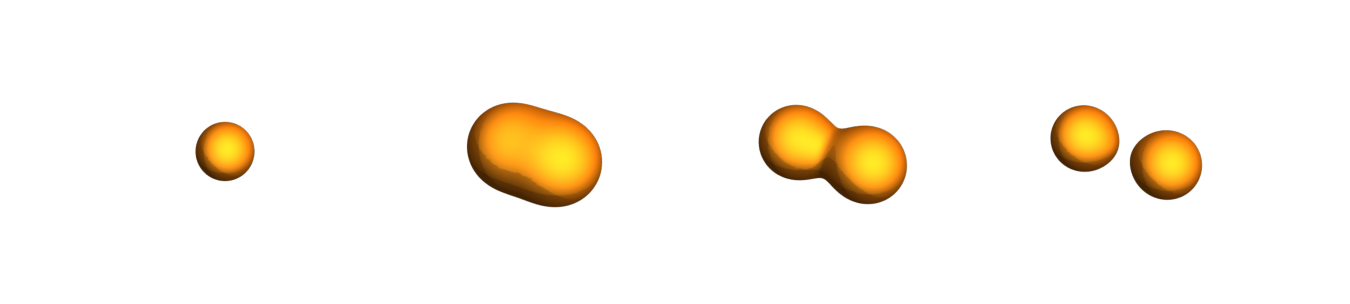
\includegraphics[width=0.8\textwidth]{images/fission-liquid-drop-split.pdf}
        \caption{A liquid drop splits in two.}
        \label{fig:liquid drop split fission}
    \end{figure}
    
    Considering \cref{fig:liquid drop split fission} we see that as the isotope begins to undergo fission the surface area increases, and hence there is an increase in surface energy.
    This is what creates the energy barrier that has to be overcome.
    As separation increases the potential energy starts to decrease as the Coulomb potential decreases.
    After the fragments split fully they repel each other and gain kinetic energy.
    
    From the liquid drop model we would assume that the favoured fission products would be two nuclei of approximately equal mass.
    However, this is not what we see.
    If we consider shell effects then we would expect that fission products with magic numbers are favoured, and this is indeed what we find.
    
    A common fission event will release approximately \qty{200}{\MeV} of energy.
    Not all of this corresponds to the kinetic energy of the daughter nuclei, there are usually other products, such as neutrons, and the nuclei produced are often in highly excited states.
    These excited states then de-excite emitting gamma rays and neutrons.
    
    \section{Induced Fission}
    It is very easy for neutrons to be absorbed by the nucleus, since they are not charged so don't have to overcome the Coulomb barrier.
    Even room temperature neutrons, with kinetic energies as low as \qty{0.025}{\MeV}, can fuse with a nucleus.
    In doing so if they fuse with, for example, \ce{^235U}, they will produce \ce{^236U}, in an excited state.
    
    \ce{^236U} can then de-excite in one of two ways.
    It can just release photons, in which case the process of neutron capture is known as \defineindex{radiative capture}.
    More interestingly, so long as the excitation energy is greater than the fission barrier height, which is \qty{6.2}{\MeV}, it can also undergo fission.
    Assuming this condition is met fission occurs rapidly, with a lifetime of approximately \(10^{-17}\,\unit{\second}\).
    
    The minimum excitation energy occurs when the kinetic energy of the neutron is zero.
    In this case the excitation energy is
    \begin{equation}
        E_{\mathrm{x}} = [M(\ce{^235U}) + m_{\Pn} - M(\ce{^{236}U})]c^2 = S_{\Pn}(^236U).
    \end{equation}
    Since \(S_\Pn(\ce{^{236}U}) = \qty{6.5}{\MeV}\) is greater than the fission barrier height, \qty{6.2}{\MeV}, it is always possible for fission to occur when \ce{^235U} captures a neutron.
    
    One problem when it comes to using uranium fission as a power source is that only \qty{0.7}{\percent} of naturally occurring uranium is \ce{^235U}.
    Most, \qty{99.3}{\percent}, is \ce{^238U}.
    The problem is that \(S_{\Pn}(\ce{^236U}) > S_{\Pn}(\ce{^239U})\), due to the additional pairing energy since \ce{^236U} is an even-even nuclei.
    This disparity is large enough that for low energy neutrons the \ce{^239U} produced by capture will not have enough energy to overcome the fission barrier, and will therefore emit photons instead.
    
    One, somewhat counter intuitive, solution is to slow down the neutrons, which can be done by elastic collisions with a moderator material, commonly graphite is used for this purpose.
    If this is done enough then the neutrons will have lower energies than the \qtyrange{1}{100}{\electronvolt} range where radiative capture has strong resonances.
    It is then more likely that \ce{^235U} will absorb the neutrons, and therefore we get fission.
    This is the process used in thermal reactors.
    It is possible to run these on un-enriched uranium, but more commonly they are run on enriched uranium, where \ce{^235U} makes up \qtyrange{2}{3}{\percent} of isotopes.
    
    The alternative solution is more obvious, and is used in what we call fast reactors.
    We simply use neutrons with energies on the order of \qty{2}{\MeV}.
    These then have enough excess energy after capture that regardless of the isotope that captures them there is enough energy to overcome the potential barrier.
    The problem with this solution is that the fission cross section is smaller at these energies and so a higher enrichment of uranium is required, approximately \qty{20}{\percent}.
    Otherwise the chain reaction can't be maintained.
    We can also use the artificial \ce{^239Pu} for this purpose, and this is often preferred, since the average number of neutrons produced per fission event is greater at this energy for \ce{^239Pu} than for \ce{^235U}.
    
    \ce{^239Pu} is not naturally occurring.
    Instead we have to create it in reactors by neutron radiative capture and then a chain of beta decays, the chain reaction, ignoring electrons and neutrinos, is
    \begin{equation}
        \Pn + \ce{^238U} \to \ce{^239U} \to \ce{^239Np} \to \ce{^239Pu}.
    \end{equation}
    Notice that this allows for the possibility of creating more fissile material within the reactor while it is running.
    
    Let \(n(t)\) be the number of neutrons at time \(t\), \(q\) be the probability that a single neutron causes fusion, and \(\nu\) be the mean number of neutrons produced per fission event.
    Then
    \begin{equation}
        \dl{n(t)} \propto (\nu q - 1)n\dd{t}.
    \end{equation}
    The solution to this is
    \begin{equation}
        n(t) = n(0)\e^{(\nu q - 1)t/\tau}
    \end{equation}
    where \(\tau\) is the mean time taken for a neutron to induce fusion.
    For pure \ce{^235U} \(\tau \approx 10^{-8}\,\unit{\second}\).
    
    For \(\nu q > 1\) this results in an exponential increase in neutron density and energy release.
    This happens for masses exceeding a critical mass, for pure \ce{^235U} a spherical sample of approximately \qty{52}{\kilogram} is sufficiently large that \(\nu\) is great enough that \(\nu q > 1\).
    We therefore have a run away exponential increase in energy release, in other words a nuclear explosion.
    Clearly this is undesirable\footnote{unless you want to kill a lot of people all at once in a pretty horrific way}.
    We say that \qty{52}{\kilogram} is the \defineindex{critical mass} for \ce{^235U}.
    
    In a reactor for a steady source of energy we need \(\nu q - 1 = 0\).
    For a typical thermal reactor \(\tau \approx 10^{-3}\,\unit{\second}\).
    This is a short time scale on which we need to control fluctuations in energy production.
    One thing that helps is that the products of fission can behave as source of delayed neutrons, for example
    \begin{equation}
        \ce{^87Br} \to \ce{^86Kr} + \Pe + \APnue + \Pn.
    \end{equation}
    This decay takes time, the lifetime of \ce{^87Br} is approximately \qty{80}{\second}.
    On these time scales we can control the number of neutrons by moving in and retracting control rods which are made of strong neutron absorbers such as \ce{B} or \ce{Cd}.
    
    %Appendicies
    %\appendixpage
    %\begin{appendices}
    %    \include{}
    %\end{appendices}
    
    \backmatter
    \begin{thebibliography}{9}
        \bibitem{lineofnuclearstability} Sjlegg, \textit{Table isotopes en}, \url{https://commons.wikimedia.org/wiki/File:Table_isotopes_en.svg}, (accessed 20/10/2021)
    \end{thebibliography}
    \renewcommand{\glossaryname}{Acronyms}
    \printglossary[acronym]
    \printindex
\end{document}
